% ------------------------------------------------------------------------------
% The OpenQuake Book 
% 
% Authors: 
% 	H. Crowley 		- Executive Committee - GEM Foundation, Pavia, Italy
%	L. Garrido 		- Executive Committee - GEM Foundation, Pavia, Italy
% 	D. Monelli 		- GEM Model Facility, Zurich, Switzerland
% 	M. Pagani 		- Executive Committee - GEM Foundation, Pavia, Italy
% 	V. Silva 		- GEM Model Facility, Pavia, Italy
%	G. Weatherhill 	- GEM Model Facility, Pavia, Italy
% 
% Document distributed under the Common Creative License 
% © GEM Foundation, Pavia, February 2011
% ------------------------------------------------------------------------------
\documentclass[12pt,a4paper,headings=small,version=first,dvips]{scrbook}
% --------------------------------------------------------------------- Packages
\setcounter{secnumdepth}{3}
\setcounter{tocdepth}{3}
%
\usepackage{pst-tree}
\usepackage{pstricks,pstricks-add,multido}

\usepackage{geometry}
\usepackage{moresize}
%
\usepackage{fancyvrb}
%
\usepackage{pbox}
%
\usepackage{makeidx} % http://en.wikibooks.org/wiki/LaTeX/Indexing
%
\usepackage{subfigure}
%
\usepackage{bm}
\makeindex
%
% - - - - - - - - - - - - - - - - - - - - - - - - - - - - - - - - Setting Fonts
\renewcommand{\encodingdefault}{OT1}
\renewcommand{\familydefault}{cmss}
\renewcommand{\seriesdefault}{m}
\renewcommand{\shapedefault}{up}
% - - - - - - - - - - - - - - - - - - - - - - - - - - - - - - - - - - - - - - -
\usepackage{amsmath}
% - - - - - - - - - - - - - - - - - - - - - - - - - - - - - - - - - - - - - - -
\usepackage{titlesec}
\usepackage[dvips]{graphicx}
% - - - - - - - - - - - - - - - - - - - - - - - - - - - - - - - - - - - - - - -
\usepackage{type1cm,eso-pic,color}
\makeatletter
\AddToShipoutPicture{
    \setlength{\@tempdimb}{.5\paperwidth}
    \setlength{\@tempdimc}{.5\paperheight}
    \setlength{\unitlength}{1pt}
    \put(\strip@pt\@tempdimb,\strip@pt\@tempdimc){
        \makebox(0,0){\rotatebox{55}{
        	\textcolor[gray]{0.85}{
        		\fontsize{5cm}{5cm}
        		\selectfont{DRAFT}}
        	}
        }
	}
}
\makeatother

% Solves problems with margin notes
\usepackage{mparhack} 
	\setlength{\marginparwidth}{1.1in}
	\let\oldmarginpar\marginpar
	\renewcommand\marginpar[1]{\-\oldmarginpar[\raggedright\color{red01}
	\footnotesize #1]%
	{\raggedright\footnotesize #1}}
% Colors
	%\definecolor{blue01}{rgb}{0,0,.5}
	\definecolor{blue01}{RGB}{4,64,116}
	\definecolor{blue02}{RGB}{0,62,113}
	\definecolor{gray01}{rgb}{0.1,0.1,0.1}
	\definecolor{gray02}{rgb}{0.8,0.8,0.8}
	\definecolor{red01}{rgb}{0.5,0.0,0.0}
	\definecolor{orange00}{rgb}{1.0,0.74,0.53}
	\definecolor{orange01}{rgb}{0.9137,0.5882,0.0980}
	\definecolor{orange02}{rgb}{0.7608,0.4157,0.1804}
	\definecolor{orange03}{rgb}{0.6941,0.1843,0.1333}
\usepackage[english]{babel}
%
\usepackage[square,colon]{natbib} % Extend bibligraphy functions

%\usepackage[labelfont=bf]{caption} % Used to reformat caption typesetting
\usepackage[textfont=it,margin=10pt,font=small,labelfont=bf, labelsep=endash]{caption}

\usepackage{scrpage2}
	\lofoot[]{
\includegraphics[width=2.0cm]{./Figures/openquake_logo1.eps}}
	\refoot[]{
\includegraphics[width=2.0cm]{./Figures/openquake_logo1.eps}}
% - - - - - - - - - - - - - - - - - - - - - - - - - -  Reformatting PART Titles
\titleformat{\part}[display]
{\filleft\normalfont\sffamily}
{\textcolor{blue01}{\bfseries\large PART}\hspace{4pt}
	\bfseries\Huge\textcolor{blue01}{\thepart}}
{1pc}
{\Huge\bfseries\textcolor{blue01}}
[]
% - - - - - - - - - - - - - - - - - - - - - - - - - Reformatting CHAPTER Titles
% Titles: CHAPTER
\titleformat{\chapter}
	[display] % shape
	{\filleft\normalfont\sffamily} % format
	{\textcolor{blue01}{\bfseries\MakeUppercase{\chaptertitlename}} % label
		\hspace{4pt}\huge\bfseries\textcolor{blue01}{\thechapter}} 
	{1pc} % sep
	{\huge\bfseries\textcolor{blue01}} % Before
	[]
% - - - - - - - - - - - - - - - - - - - - - - - - - Reformatting SECTION Titles
% Titles: SECTION
\titleformat{\section}
	[hang] % shape
	{\vspace{.8ex}\Large\bfseries\color{blue01}} % format 
	{\textcolor{blue01}{\thesection.}} % label
	{.5em} % sep
	{} % before
	[] % after
% - - - - - - - - - - - - - - - - - - - - - - -  Reformatting SUBSECTION Titles
% Title: SUBSECTION
\titleformat{\subsection}
	[hang] % shape
	{\vspace{.8ex}\large\bfseries\color{blue01}} % format 
	{\textcolor{blue01}{\thesubsection.}} % label
	{.5em} % sep
	{} % before
	[] % after
%  - - - - - - - - - - - - - - - - - - - - -  Reformatting SUBSUBSECTION Titles 
% Title: SUBSUBSECTION
\titleformat{\subsubsection}
	[hang] % shape
	{\vspace{.8ex}\normalfont\bfseries\color{blue01}} % format 
	{\textcolor{blue01}{\thesubsubsection.}} % label
	{.5em} % sep
	{} % before
	[] % after
% - - - - - - - - - - - - - - - - - - - - - - -  Reformatting PARAGRAPH Titles 
% Title: PARAGRAPH
\titleformat{\paragraph}
	[hang] % shape
	{\vspace{.8ex}\normalfont\bfseries\color{blue01}} % format 
	{} % label
	{.5em} % sep
	{} % before
	[] % after
%
% ------------------------------------------------------------------------------
\uppertitleback{
   \textbf{Authors:} \\
   Helen Crowley$^1$, Leonardo Garrido$^1$, Damiano Monelli$^3$, 
   Marco Pagani$^1$, Vitor Silva$^2$, Graeme Weatherill$^2$ \\ \hfill \\
   \small
   $^1$ GEM Foundation\\
   via Ferrata, 1 \\ 
   20133 Pavia \\
   Italy \\
   \hfill\\
   $^2$ GEM Model Facility\hfill\\
   via Ferrata, 1\hfill\\ 
   20133 Pavia\hfill\\
   Italy\hfill\\
   \hfill\\
   $^3$ GEM Model Facility\hfill\\
   SED - ETHZ\hfill\\ 
   Sonneggstrasse, 5\\
   CH-8092 Zurich\hfill\\
   Switzerland \hfill\\ 
   \hfill\\
   Email address (for all the authors):\hfill\\
   $<$name.surname$>$@globalquakemodel.org
   \normalsize
}  
%
% =============================================================== BEGIN DOCUMENT
% -------------------------------------------------- Title and table of contents
\begin{document}
% - - - - - - - - - - - - - - - - - - - - - - - - - - - - - - - - - - - -  Cover
\newgeometry{hmargin={-0.4cm,0cm},height=29.7cm}
\thispagestyle{empty}
\psset{unit=1cm}
\begin{pspicture}(0,0)(21cm,29.7cm)
	\psframe[fillstyle=solid,linecolor=white,fillcolor=white]
		(0.0cm,15.0cm)(21cm,29.7cm)	
	\rput[l](0cm,15cm){\includegraphics[width=21cm,height=15cm]{./Figures/adapazari.eps}}
	\psframe[fillstyle=solid,linecolor=gray02,fillcolor=gray02]
		(0.0cm,0.0cm)(21cm,15.1cm)
	
	\psframe[fillstyle=solid,linecolor=orange01,fillcolor=orange01]
		(0.0cm,15.0cm)(21cm,15.5cm)
%	\psframe[fillstyle=solid,linecolor=blue02,fillcolor=blue02]
%		(0.0cm,15.6cm)(21cm,15.75cm)
	\psframe[fillstyle=solid,linecolor=orange01,fillcolor=orange01]
		(0.0cm,25.0cm)(21cm,25.1cm)
%	\psframe[fillstyle=solid,linecolor=blue02,fillcolor=blue02]
%		(0.0cm,25.15cm)(21cm,25.18cm)
	%
	\rput[r](19.5cm,13.5cm){\sffamily\bfseries\HUGE\color{orange01}
		{The OpenQuake Book}}
	%\rput[r](19cm,19.5cm){\sffamily\Large\color{gray02}{\emph{Shaken not stirred}}}
	% Old Version
	%\rput[r](18cm,22cm){\sffamily\bfseries\HUGE\color{blue02}
	%	{The OpenQuake Book}}
	%\rput[r](18cm,21cm){\sffamily\Large\color{gray02}{\emph{Shaken not stirred}}}
	% 
	\rput(4cm,27.5cm){
\includegraphics[height=1.5cm]
		{./Figures/openquake_logo1.eps}}
	%
%	\rput[r](18cm,27.5cm){\includegraphics[height=1.5cm]
%		{./Figures/GEM_logo.eps}}
	%\rput[r](18cm,9cm){\includegraphics[width=15cm]{./Figures/adapazari.eps}}
	\rput[r](19.5cm,2cm){\sffamily\large\color{gray01}{Version 1.0}}
\end{pspicture}
%  - - - - - - - - - - - - - - - - - - - - - - - - - - - - - - - - - Second page
\restoregeometry
%
% - - - - - - - - - - - - - - - - - - - - - - -  This is the internal title page
\setcounter{page}{1}
\begin{titlepage}
	\titlehead{\emph{``OpenQuake: Shaken not stirred''}}
	\title{ \textcolor{blue01}{\textsf{\bfseries\Huge The OpenQuake Book}}  }
	\date{}
\end{titlepage}
\pagestyle{scrheadings}
\maketitle
\tableofcontents
%
% --------------------------------------------------------- Symbols and acronyms
\chapter*{Symbols and acronyms}
	\begin{tabular}{p{9.5cm}rr}
\bf{Quantity or Description} & \bf{Symbol or} & \bf{Unit of} \\ 
              & \bf{acronym}   & \bf{measure}  \\
Distance \dotfill & $D$ or $d$ & \text{km} \\ 
Frequency-Magnitude Distribution \dotfill & FMD & \\
Gutenberg-Richter (frequency-magnitude distribution) \dotfill & G-R &  \\
Ground motion (GM) or intensity measure type (IMT) \dotfill & $U$ or $u$ & g \\
Ground Motion Field \dotfill & GMF & \\
Ground Motion Prediction Equation \dotfill & GMPE &  \\
Ground Motion Prediction Equation System \dotfill & GMPES &  \\
Magnitude \dotfill & $M$ or $m$ & \\
Natural hazards' Risk Markup Language \dotfill & nrML & \\
Occurrence Rate \dotfill & $\lambda$ & events/yr \\
OpenQuake \dotfill & OQ & \\
Rupture \dotfill & $rup$ & \\
Seismic Source System \dotfill & SSS \\
Stochastic Event Set \dotfill & SES & \\
\end{tabular}

% ==============================================================================
% ------------------------------------------------------------------------- Part
\part{Introduction}
% ------------------------------------------------------------------------------
\chapter{OpenQuake background}
	This book aims to provide an explanation of the scientific basis 
and the methodologies adopted in the implementation of OpenQuake, an open 
source code for seismic hazard and risk calculation. 
%
The book follows the traditional openness and transparency features of the 
\gls{acr:gem} as clearly indicated in the development principles of 
OpenQuake. 

%
The \gls{acr:gem} initiative aims at establishing uniform, open 
standards to calculate and communicate earthquake risk worldwide, by 
developing together with the community a global, state-of-the-art and 
dynamic earthquake risk model. 
%
OpenQuake is a fully integrated, flexible and scalable hazard and risk 
calculation engine whose development is at the core of \gls{acr:gem}'s
overall objectives.
% ------------------------------------------------------------------------------
\section{The Basics of OpenQuake}
The implementation of OpenQuake officially started in Summer 2010 
following the experience gained in \gls{acr:gem}'s kick-off project GEM1 
\citep{gemfoundation2010}, during which an extensive appraisal of existing hazard 
and risk codes was performed \citep{danciu2010,crowley2010}
and prototype hazard and risk software were selected, designed and
implemented \citep{pagani2010,crowley2010a}.

Currently OpenQuake is a blend of Java and Python code developed 
following the most common requirements of Open Source 
software development, such as a public repository, IRC channel and open mailing lists. 
The source code, released under an open source software license,
is freely and openly accessible on a web based repository 
(see \href{http://github.com/gem}{github.com/gem}) while the 
development process is managed so that the community can participate 
to the day by day development as well as in the mid- and long-term 
design process. 
%
OpenQuake development also leverages from a number of open source projects 
such as \href{http://www.opensha.org}{OpenSHA}, \href {http://celeryproject.org}{Celeryd} and \href{http://www.rabbitmq.com}{RabbitMQ}, just to mention a few.

The hazard component of the engine, which constitutes almost entirely
the Java part of the code, largely relies on classes belonging to 
\gls{opensha}, a comprehensive library for performing state-or-the-art
PSHA developed collaboratively at the \gls{acr:usgs} and at the 
\gls{acr:scec}. New code was developed in GEM1 and in the following 
phases to support a standardized \gls{acr:erf} and logic-tree structure, 
event-based PSHA and, seismic hazard disaggregation.
%
The Risk component of the engine was designed in GEM1, prototyped in Java and eventually
coded in Python by the OpenQuake team operating at the \gls{acr:gem} 
Model Facility.

A schema that illustrates OpenQuake's structure is 
represented in Figure \ref{fig:openquake_schema}; the schema contains:
purple boxes representing the main modules of the hazard component, 
green boxes showing the modules of the risk component, white boxes
with main outputs computed by the distinct modules and orange rectangles
displaying the main input information that should be entered into the calculation engine. 
%
% ------------------------------------------------------------------------------
%\subsection{Brief description of the OpenQuake IT architecture}
%% ------------------------------------------------------------------------------
Openquake is the core of the OpenGEM system. 

As it appears in Figure \ref{fig:oq_it}, OpenQuake is powered by a 
number of open source software projects, of which OpenSHA-lite and 
RiskLib are currently the most essential ones. 
OpenSHA-lite is a ‘light’ version of the comprehensive software for 
probabilistic seismic hazard assessment OpenSHA and whose code serves
as a basis for the hazard component of the OpenQuake engine. RiskLib 
is a global collaboration project that is aimed at common development 
of a code ‘library’ for the risk all types of natural hazards, including
an API, on wh ich ‘apps’ can be built, such as tools that support risk
mitigation/reduction. The World Bank’s GFDRR, OpenGeo, AIFDR and GEM 
jointly work on RiskLib and its code repository, currently part of 
the OpenQuake project, will be broken out soon.

Implementation of a standard format for data exchange for natural hazard
and risk,  is closely related to what is described above. The NRML 
(Natural hazards’ Risk Markup Language) format has been developed, which
is capable of encompassing a wide variety of risk and hazard data formats.
More information can be found in the detailed background documentation 
for OpenQuake.

The data services that are mentioned above are globally accessible 
read/write collaborations of core data sets that are exposed with a 
REST API. Some of the core modules of GEM will be available through 
the services and are currently being developed by GEM’s Model Facility 
development team, in collaboration with a number of IT partners and the 
scientists coordinating the modules. Examples are the development of a 
global exposure database, development of a global portal for active 
faults, global vulnerability functions and an earthquake consequences
database.
% . . . . . . . . . . . . . . . . . . . . . . . . . . . . . . . . . . . > Figure
\begin{figure}
\includegraphics[width=20cm,angle=0]{./Figures/Part_Introduction/engine9_20110130.eps}
\caption{xx}
\label{fig:oq_it}
\end{figure}
% . . . . . . . . . . . . . . . . . . . . . . . . . . . . . . . . . . . < Figure




%
% ------------------------------------------------------------------------------
\section{Book structure}
The OpenQuake book is organized into three parts; in the first we give
a broad introduction to OpenQuake and the Book, in the second we 
describe the science behind the hazard component of the engine
whilst in the third we illustrate the theory of the risk calculators
incorporated into OpenQuake.

\hfill \\
\emph{Part II: Hazard}
\begin{itemize}
\item Chapter \ref{chap:inthaz} offers an introduction to the hazard 
topics discussed in the following chapters. In particular, in this 
Chapter we discuss the main OpenQuake concepts and we illustrate the 
calculation workflows currently available in the hazard component of 
OpenQuake.
\item Chapter \ref{chap:hazinp} focuses on the structure and the 
characteristics of the information necessary to define a 
comprehensive PSHA input model. This Chapter also includes
descriptions of the main seismic source typologies and of the logic 
tree structure.
\item We dedicate Chapter \ref{chap:erf} to the explanation of the
methodology adopted for the processing of the logic tree structures
supported by OpenQuake and for the creation of the 
\gls{earthquakeruptureforecast}
\item The last Chapter of the hazard part (chapter \ref{chap:hazcalc}) 
illustrates the main calculators available: the classical-PSHA calculator,
the event-based calculator and the disaggregation calculator. 
\end{itemize}
\emph{Part III: Risk}
\begin{itemize}
\item Chapter \ref{chap:intrisk} introduces the main risk concepts and workflows. 
\item Chapter \ref{chap:riskinput} contains an explanation of the exposure, 
physical vulnerability and fragility concepts.
\item Chapter \ref{chap:risk_deterministic} describes the deterministic event-based risk 
methodology implemented in \gls{acr:oq}.
\item Chapter \ref{chap:risk_prob_event_based} provides an overview of the 
probabilistic event-based risk calculation methodology.
\item Chapter \ref{chap:risk_psha_based} illustrates risk calculations based on 
the hazard curves from classical PSHA.
\end{itemize}
%
In the closing part, the Book contains a glossary that aims to define a 
clear and unique terminology.
%
% . . . . . . . . . . . . . . . . . . . . . . . . . . . . . . . . . . . > Figure
\begin{landscape}
\begin{figure}
\includegraphics[width=20cm,angle=0]{./Figures/Part_Introduction/engine9_20110130.eps}
\caption{OpenQuake schema. Purple boxes are the calculators included in the  
the hazard part of OQ; green boxes are the risk calculators. The method of 
\citet{wesson2009} (not currently supported) is represented in a separate box since it incorporates 
hazard and risk calculations.}
\label{fig:openquake_schema}
\end{figure}
\end{landscape}
% . . . . . . . . . . . . . . . . . . . . . . . . . . . . . . . . . . . < Figure
% ------------------------------------------------------------------------------
\chapter{Brief desciption of OpenQuake IT aspects}
	% ------------------------------------------------------------------------------
Openquake is the core of the OpenGEM system. 

As it appears in Figure \ref{fig:oq_it}, OpenQuake is powered by a 
number of open source software projects, of which OpenSHA-lite and 
RiskLib are currently the most essential ones. 
OpenSHA-lite is a ‘light’ version of the comprehensive software for 
probabilistic seismic hazard assessment OpenSHA and whose code serves
as a basis for the hazard component of the OpenQuake engine. RiskLib 
is a global collaboration project that is aimed at common development 
of a code ‘library’ for the risk all types of natural hazards, including
an API, on wh ich ‘apps’ can be built, such as tools that support risk
mitigation/reduction. The World Bank’s GFDRR, OpenGeo, AIFDR and GEM 
jointly work on RiskLib and its code repository, currently part of 
the OpenQuake project, will be broken out soon.

Implementation of a standard format for data exchange for natural hazard
and risk,  is closely related to what is described above. The NRML 
(Natural hazards’ Risk Markup Language) format has been developed, which
is capable of encompassing a wide variety of risk and hazard data formats.
More information can be found in the detailed background documentation 
for OpenQuake.

The data services that are mentioned above are globally accessible 
read/write collaborations of core data sets that are exposed with a 
REST API. Some of the core modules of GEM will be available through 
the services and are currently being developed by GEM’s Model Facility 
development team, in collaboration with a number of IT partners and the 
scientists coordinating the modules. Examples are the development of a 
global exposure database, development of a global portal for active 
faults, global vulnerability functions and an earthquake consequences
database.
% . . . . . . . . . . . . . . . . . . . . . . . . . . . . . . . . . . . > Figure
\begin{figure}
\includegraphics[width=20cm,angle=0]{./Figures/Part_Introduction/engine9_20110130.eps}
\caption{xx}
\label{fig:oq_it}
\end{figure}
% . . . . . . . . . . . . . . . . . . . . . . . . . . . . . . . . . . . < Figure



% ==============================================================================
% ------------------------------------------------------------------------- Part
\part{Hazard}
% ------------------------------------------------------------------------------
\chapter{Introduction}
	\label{chap:inthaz}
	Probabilistic Seismic Hazard is nowadays a well established methodology, largely founded on the works of \citeauthor{cornell1968} and \citeauthor{esteva1968}, both published at the end of the 1960's. 
%
The development of PSHA within the latest four decades did not change much the original concept but made calculations more rigorous and accurate, especially with respect to treatment of uncertainties. 
%
The evolution of PSHA methodologies proceeded in parallel with the development of instrumental seismology and computing hardware. USGS and UNAM covered an important role in the development of PSHA. Computer codes such as EQRISK \citep{mcguire1976} and different SEISRISK versions \citep{bender1982,bender1987} traced the advancement of PSHA calculation within
the last part of the 20th century.
% 
Nowadays the most computationally intensive PSHA models available are the ones developed for site-specific PSHA analyses, such as the ones performed for special installations, and the regional PSHA input models. In the first case most of the demand comes from the complexity of the input whilst in the second case is the number of sites considered that makes calculation heavy.  
%
% ------------------------------------------------------------------------------
\section{OpenQuake-hazard}
OpenQuake-hazard leverages from OpenSHA (http://www.opensha.org) - an open-source, Java-based platform for conducting Seismic Hazard Analysis - and it is developed in collaboration with the OpenSHA team. 
% ------------------------------------------------------------------------------
\chapter{OpenQuake input description}
	\label{chap:hazinp}
	An OpenQuake PSHA input model contains four distinct information blocks: 
(1) information 
regarding location, geometry, and seismicity generation properties of seismic
sources, (2) information about ground motion prediction equations to be 
adopted in the calculation, (3) information about the epistemic uncertainties 
related to the two aforementioned points, and (4) information specifying 
calculation settings.

The description of epistemic uncertainties is accomplished via a logic-tree 
structure, described branching level by branching level. In OpenQuake it's 
possible to define two logic-tree structures: one describing epistemic 
uncertainties associate with the creation of the ERF and one considering the
uncertainties connected with the use of GMPEs. For the sake of homogeneity 
and simplicity, the OpenQuake PSHA input models are always defined using two 
logic tree structures. In cases when epistemic uncertainties are non accounted
for, the two logic tree structures simply have one branching level with one 
branch (with weight equal to 1).
Further explanations on the way we describe and model logic-tree is provided 
in section \ref{hazard:logic_tree} at page \pageref{hazard:logic_tree}. 

The description of OpenQuake seismic source properties is subdivided into 
source location and geometry and source frequency-magnitude distribution. 
Section \ref{hazard:seismic_source_types} provides an in deep description of 
the properties pertinent to the different source types supported, together 
with examples of each single source type nrML description. 

The selection of ground motion prediction equations (GMPE) in OpenQuake 
is basically accomplished by specifying a label in a particular file.  
The user can associate a GMPE to each tectonic region considered in the 
analysis (Active Shallow tectonic, Stable Continental etc.). Examples of 
GMPEs selection are provided in section \ref{hazard:gmpe_selection} at page 
\pageref{hazard:gmpe_selection}.

The last, but not less important, block of information characterizing a PSHA 
input model contains parameters specifying the way calculations must be 
carried out. The information to be included in this part of the input is 
strictly related to the calculation properties of the engine. Section 
\ref{hazard:calculation_settings} provides an outlook of the hazard specific 
calculation setting supported by OpenQuake. 
%
% ------------------------------------------------------------------------------
\section{Logic-tree description}
\label{hazard:logic_tree}
Logic-trees are a tool designed to consider in a systematic manner the 
epistemic uncertainties of models and parameters included in a hazard 
analysis.

In OpenQuake, the description of a logic-tree structure uses as its principal 
component a branching level where a branching level consists on (1) the 
definition of the parameter - or model - affected by uncertainty, (2) the 
specification of the type of uncertainty (3) the listing of the - mutually 
exclusive and collectively exhaustive \citep{bommer2008} - alternative 
hypotheses and, (4) the index of the branches of the previous level to which 
this branching level applies. 
Each hypothesis (i.e. branch) included in a branching level has 
an associated value and a corresponding weight expressing - according to 
different interpretations available in the literature - ``probabilities or 
simply subjective indications of relative merit'' 
\citep[][pagecon 999]{bommer2008}.

Figure \ref{fig:logic_tree_branching_levels} depicts a 
branching level defining epistemic uncertainties on the dip angle of simple 
fault sources. In this case the possible values of the dip are specified
on each branch composing the branching level (i.e. 30, 45 and 60 degrees). This 
means that these three values are the only ones admitted for all the sources 
included in the Source Model considered in this example. 
% . . . . . . . . . . . . . . . . . . . . . . . . . . . . . . . . . . . > Figure
\renewcommand{\psedge}{\ncdiag[armA=0,angleB=180,armB=1cm]}
\begin{figure}[!hb]
%\fbox{\begin{minipage}{\textwidth}
\hfill \\
\textcolor{blue01}{\emph{Branching level definition}}: \dotfill Simple Fault 
	Dip Angle \\
\textcolor{blue01}{\emph{Branching level uncertainty type}}: \dotfill 
	Absolute values \\
\textcolor{blue01}{\emph{Applies to}}: \dotfill Simple faults \\
\textcolor{blue01}{\emph{Correlated branches}}: \dotfill Yes \\
\hfill \\
	\centering
	\begin{psTree}[treemode=R,levelsep=*2cm]
			{\Tr{ }}
		\begin{psTree}[treemode=R]{
			\Tr{\parbox[b]{4cm}{ value = 30$^\circ$ 
				\newline weight=w$_1$}}}%
		\end{psTree}%
		\begin{psTree}[treemode=R,treenodesize=1cm]{
			\Tr{\parbox[b]{4cm}{ value = 45$^\circ$ 
				\newline weight=w$_2$}}}%
		\end{psTree}%
		\begin{psTree}[treemode=R]{
			\Tr{\parbox[b]{4cm}{ value = 60$^\circ$ 
				\newline weight=w$_3$}}}%
		\end{psTree}%
	\end{psTree}%
\\ \hfill \\
%\end{minipage}} % End of fbox
\caption{Branching level description example. The upper example shows a 
branching level describing epistemic uncertainties on faults dip angle}
\label{fig:logic_tree_branching_levels}
\end{figure}
% . . . . . . . . . . . . . . . . . . . . . . . . . . . . . . . . . . . < Figure
%

As in the case of Figure \ref{fig:logic_tree_branching_levels},  
Figure \ref{fig:logic_tree_branching_levels_1} also shows a branching level 
defining epistemic uncertainties on the dip angle of simple fault sources.
However - contrary to the example in Figure 
\ref{fig:logic_tree_branching_levels}, in this case the values specified for 
each branch aren't absolute dip angles but instead delta values to be added - 
or subtracted - to the initial dip value specified for each simple fault source
inclued in the initial source model.

% . . . . . . . . . . . . . . . . . . . . . . . . . . . . . . . . . . . > Figure
\renewcommand{\psedge}{\ncdiag[armA=0,angleB=180,armB=1cm]}
\begin{figure}
%\fbox{\begin{minipage}{\textwidth}
\hfill \\
\textcolor{blue01}{\emph{Branching level definition}}: \dotfill
	Simple Fault Dip Angle \\
\textcolor{blue01}{\emph{Branching level uncertainty type}}: \dotfill
	Relative values \\
\textcolor{blue01}{\emph{Applies to}}: \dotfill
	All previous branches \\
\textcolor{blue01}{\emph{Correlated branches}}: \dotfill Yes \\
\hfill \\
	\centering
	\begin{psTree}[treemode=R,levelsep=*2cm]
			{\Tr{ }}
		\begin{psTree}[treemode=R]{
			\Tr{\parbox[b]{4cm}{ value = -15$^\circ$ 
				\newline weight=w$_1$}}}%
		\end{psTree}%
		\begin{psTree}[treemode=R,treenodesize=1cm]{
			\Tr{\parbox[b]{4cm}{ value = 0$^\circ$ 
				\newline weight=w$_2$}}}%
		\end{psTree}%
		\begin{psTree}[treemode=R]{
			\Tr{\parbox[b]{4cm}{ value = +15$^\circ$ 
				\newline weight=w$_3$}}}%
		\end{psTree}%
	\end{psTree}%
\\ \hfill \\
%\end{minipage}} % End of fbox
\caption{Branching level description example. The upper example shows a 
branching level describing epistemic uncertainties on faults dip angle}
\label{fig:logic_tree_branching_levels_1}
\end{figure}
% . . . . . . . . . . . . . . . . . . . . . . . . . . . . . . . . . . . < Figure
%
Once a set of branching levels are defined, they can be easily and flexibly 
combined to create an entire logic-tree structure.
	\marginpar{marco: we probably need abstract classes for all these 
	components of the LT structure}
Figure \ref{fig:logic_tree_schema} shows an example of a logic tree structure 
obtained by combining two distinct branching levels.  

%
% . . . . . . . . . . . . . . . . . . . . . . . . . . . . . . . . . . . > Figure
\begin{figure}
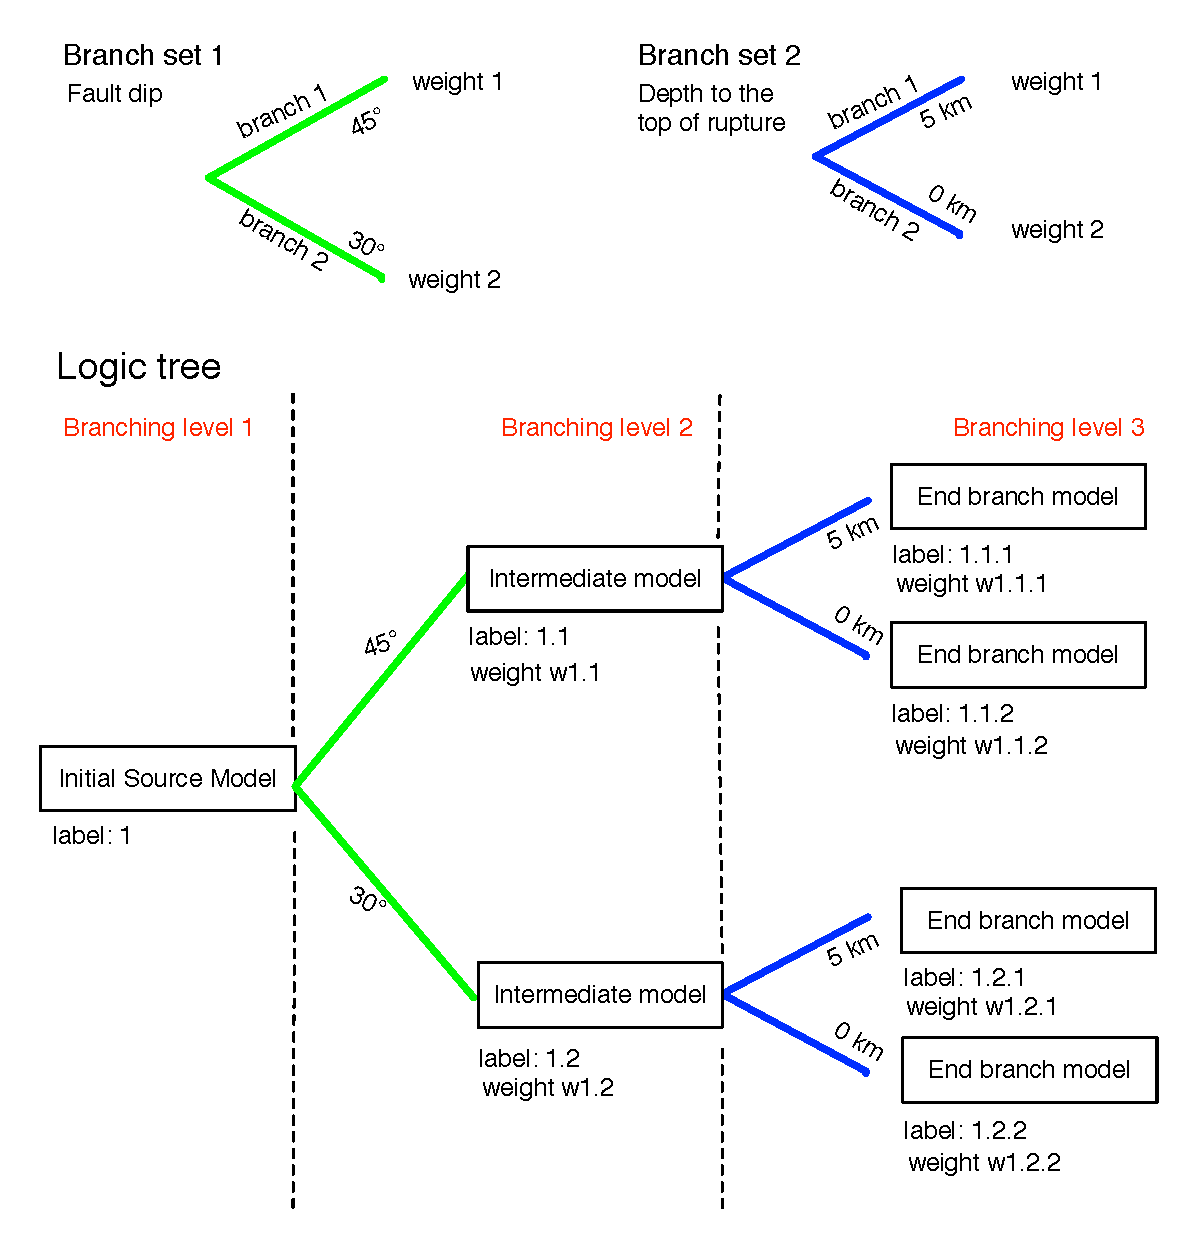
\includegraphics[width=15cm]{./Figures/Part_Hazard/logic_tree_schema.eps}
\caption{Example of a logic tree structure as defined in OpenQuake. The upper
part of the Figure depicts two branching levels.}
\label{fig:logic_tree_schema}
\end{figure}
% . . . . . . . . . . . . . . . . . . . . . . . . . . . . . . . . . . . < Figure
%

Figure \ref{fig:nrMl_logic_tree_example} shows an example of a nrML file 
describing the logic tree structure.
%
% . . . . . . . . . . . . . . . . . . . . . . . . . . . . . . . . . . . > Figure
\begin{figure}[!ht]
\small
\begin{Verbatim}[numbers=left,frame=single,fontsize=\small]
<?xml version="1.0" encoding="UTF-8"?>
<ns2:logicTreeSet 
 xmlns:ns1="http://www.opengis.net/gml/profile/sfgml/1.0"
 xmlns:ns2="http://openquake.org/xmlns/nrml/0.1"
 xmlns:ns3="http://www.w3.org/1999/xlink"
 xmlns:xsi="http://www.w3.org/2001/XMLSchema-instance"
 xsi:schemaLocation="http://openquake.org/xmlns/nrml/0.1 
    file:/Users/damianomonelli/Projects/opengem/docs/schema/nrml_seismic.xsd">
    <ns2:logicTree tectonicRegion="Active Shallow Crust">
        <ns2:logicTreeBranchSet ns2:uncertaintyType="gmpeModel">
            <ns2:logicTreeBranch>
                <ns2:uncertaintyModel>
                    BA_2008_AttenRel
                </ns2:uncertaintyModel>
                <ns2:uncertaintyWeight>0.5</ns2:uncertaintyWeight>
            </ns2:logicTreeBranch>
            <ns2:logicTreeBranch>
                <ns2:uncertaintyModel>
                    CB_2008_AttenRel
                </ns2:uncertaintyModel>
                <ns2:uncertaintyWeight>0.5</ns2:uncertaintyWeight>
            </ns2:logicTreeBranch>
        </ns2:logicTreeBranchSet>
    </ns2:logicTree>
    <ns2:logicTree tectonicRegion="Subduction Interface">
        <ns2:logicTreeBranchSet ns2:uncertaintyType="gmpeModel">
            <ns2:logicTreeBranch>
                <ns2:uncertaintyModel>
                    McVerryetal_2000_AttenRel
                </ns2:uncertaintyModel>
                <ns2:uncertaintyWeight>1.0</ns2:uncertaintyWeight>
            </ns2:logicTreeBranch>
        </ns2:logicTreeBranchSet>
    </ns2:logicTree>
</ns2:logicTreeSet>
\end{Verbatim}
\normalsize
\caption{nrML example}
\label{fig:nrMl_logic_tree_example}
\vspace*{1em}
\end{figure}
% . . . . . . . . . . . . . . . . . . . . . . . . . . . . . . . . . . . < Figure
%
% ------------------------------------------------------------------------------
\section[The OpenQuake source model]{The OpenQuake source model - Description 
of input data pertinent to the creation of the ERF}
%
The creation of the Earthquake Rupture Forecast (or seismicity probabilistic 
occurrence model) is the first step in the calculation of hazard following a 
probabilistic procedure. 

As mentioned in the introductory part of this Chapter, information describing 
the input data for the creating the ERF in OpenQuake is always organized into 
a logic tree structure.
%
%  - - - - - - - - - - - - - - - - - - - - - - - - - - - - - - - - - - - - - - -
\subsection{Seismic source typologies description}
\label{hazard:seismic_source_types}
%
OpenQuake, at present time, provides four seismic source typologies, for the 
most part defined in the course of the GEM1 project \citep{pagani2010}:
\begin{itemize}
\item Area source - This source type is the one that - at least for the time 
being - is most frequently adopted in national and regional PSHA models.
\item Grid source - Grid sources can be considered a replacement for area 
sources since they both model distributed seismicity;
\item Simple fault sources - Simple faults are the easiest modality available
to specify the parameters need to characterize a fault source. This typology
is usually adopted to describe shallow seismogenic fault sources.
\item Complex fault sources - Complex faults is usually adopted to model
subduction interface sources with a complex geometry. 
\end{itemize}

The basic assumptions adopted in the definition of these source typologies 
are the following:
\begin{itemize}
\item In the case of area and fault sources, the seismicity is homogeneously 
distributed over the source; 
\item Seismicity temporal occurrence follows a Poissonian model; 
\item The frequency-magnitude distribution can be approximated to a evenly 
discretized distribution. 
\end{itemize}
%
%  . . . . . . . . . . . . . . . . . . . . . . . . . . . . . . . . . . . . . . . 
\subsubsection{Area sources}
\label{hazard:seismic_source_types:areaSources}
Area sources usually model the seismicity occurring over wide areas where fault 
sources identification or characterization - i.e. the unambiguous definition 
of seismicity occurrence parameters - is difficult. 

The \citet{sshac1997} defined three main types of area seismic sources using as 
a discriminant their extension:
\begin{enumerate}
\item Area sources enclosing concentrated zones of seismicity;
\item Regional area sources;
\item Background area sources.
\end{enumerate}
As a general rule, the criteria - and the related uncertainties - adopted for 
their definition varies according to each area source type. From a hazard 
computation standpoint we do not introduce any difference between these three 
area types.
	\marginpar{marco: In the future we may support a specialized background 
	area source type}
%
%  . . . . . . . . . . . . . . . . . . . . . . . . . . . . . . . . . . . . . . . 
\paragraph{Parameters}
\begin{itemize}
\item A polygon that identifies the external border of the area. Eventually, 
internal borders can be specified so as to create holes inside an area.
	\marginpar{marco: I don't think nrML supports area sources with holes.}
\item One (or many) couples of the following objects:
\begin{itemize}
	\item A discrete Frequency-Magnitude Distribution (FMD)
	\item Strike, dip, and rake angles characterizing the seismicity specified 
	in the associated FMD and occurring in the area source under consideration. 
	For example, \cite{coppersmith2009} defines a discrete 
	distribution of strike values (dip is not considered because the source-site 
	metrics they use is the Joyner-Boore distance). 
\end{itemize}
This area source specification permits the accurate characterization of 
seismicity occurrence within an area by explicitly distributing the seismicity 
on the existing faulting trends. 
\item An array to specify the depth to the top of rupture dependency on magnitude. 
The array contains two columns and one or many $<$depth, magnitude$>$ tuples. 
Each tuple specifies the depth to the top of rupture for magnitudes equal or 
greater than the specific value. 
\item A value to indicate the hypocentral depth in case of punctual sources. 
By convention all the events with magnitude lower than the lowest value contained 
in the array used to specify the depth to the top of rupture are modelled 
considering a punctual source. On the opposite, ruptures with magnitude equal or 
greater than the lowest value of magnitude contained in the depth to the top of 
rupture array are modelled considering their finite dimensions. 
\end{itemize}
%
%  . . . . . . . . . . . . . . . . . . . . . . . . . . . . . . . . . . . . . . .
\subsubsection{Grid sources}
A grid source is a typology used to model distributed seismicity - usually 
of low and intermediate magnitude.

Grid sources can be considered as a PSHA source model alternative to area 
sources since they both try to represent distributed seismicity. Grid sources 
usually derive from the application of seismicity smoothing algorithms 
\citep{frankel1995,woo1996}. 

The use of these algorithms carries some advantages compared to area sources, 
indeed, (1) they remove most of the unavoidable degree of subjectivity due to 
the definition of the geometries and (2) they define a seismicity spatial 
pattern that is, usually, more similar to reality. Nevertheless, some smoothing 
algorithms require the a-priori definition of some setup parameters that expose 
the calculation to a certain partiality level.

Grid source models are modelled in OpenQuake simply as set of 
point sources. The next section describes the parameters required to 
characterize a point source.
%
%  . . . . . . . . . . . . . . . . . . . . . . . . . . . . . . . . . . . . . . . 
\paragraph{Parameters}
%
For each grid node:
\begin{itemize}
\item A location specified in terms of the <latitude,longitude> tuple;
\item Similarly to area sources, one (or many) couples of the following objects:
	\begin{itemize}
	\item A discrete Frequency-Magnitude Distribution (FMD)
	\item Strike, dip, and rake angles characterizing the seismicity specified 
	in the associated FMD. 
	\end{itemize}
\item An array to specify the dependency on magnitude of the depth to the top of 
	rupture. This array contains two columns and one or many 
	$<$depth, magnitude$>$ tuples where each tuple specifies the depth to the 
	top of rupture for magnitudes equal or greater than a specific value. 
\item A value to indicate the hypocentral depth in case of punctual sources. The 
	same convention specified for area sources applies here. 
\end{itemize}
%  - - - - - - - - - - - - - - - - - - - - - - - - - - - - - - - - - - - - - - - -
\subsection{Accounting for rupture finiteness in case of areal and grid sources}
%
In the scientific literature is well known that for magnitudes approximately 
greater than six the finite dimension of the rupture cannot be neglected in 
the calculation of the source-site distance. 
	\marginpar{marco: we need at least one citation}
	\marginpar{marco: it's not clear if and how much ruptures can extend
	outside the area border}

To correctly calculate the source-site distance in case of area and grid sources 
two are the approaches available. The first is to multiply the epicentral or 
hypocentral distance by a correction factor (see for example \cite{harmsen2008})
the second requires to place on each node a number of ruptures with different 
orientation. 
%
%  . . . . . . . . . . . . . . . . . . . . . . . . . . . . . . . . . . . . . . .
\subsubsection{Simple faults}
%
Simple Faults are the most common source type used to model faults; the 
``simple'' adjective here refers to the geometry description of the source 
which is basically obtained by projecting a trace along a representative dip 
direction. 
%
%  .   .   .   .   .   .   .   .   .   .   .   .   .   .   .   .   .   .   .   . 
\paragraph{Parameters}
%
\begin{itemize}
\item A fault trace (usually a multi-segment line) 
\item A FMD 
\item A representative value of the dip angle (Aki-Richards convention; see 
	\citet{aki2002}),
\item Rake angle (Aki-Richards convention; see \citet{aki2002}) 
\item Upper and lower values of depth limiting the seismogenic interval 
\item A boolean flag that specifies if ruptures should follow a magnitude scaling 
relationship and thus be distributed homogeneously over the fault surface or it is 
accepted that ruptures of whatever magnitude (of course of the ones admitted by 
the FMD) will rupture the whole fault surface.
\end{itemize}
%
%  . . . . . . . . . . . . . . . . . . . . . . . . . . . . . . . . . . . . . . .
\subsubsection{Complex faults}
%
Complex faults differ from simple fault just by the way geometry is described and, 
consequently in the way the fault surface is created. The input parameters used to 
describe complex faults are, for the most part, the same used to describe the 
simple fault typology. In particular, in the case of complex faults the dip angle
is not requested while the fault trace is substituted by two fault traces used to 
limit at top and bottom the fault surface. 
%
%  .   .   .   .   .   .   .   .   .   .   .   .   .   .   .   .   .   .   .   . 
\paragraph{Representation of complex faults}
%
Usually, we use complex faults to model intraplate megathrust faults such as the 
big subduction structures active in the Pacific (Sumatra, South America, Japan).

%
% ------------------------------------------------------------------------------
\section{GMPEs description}
\label{hazard:gmpe_selection}
%

%
% ------------------------------------------------------------------------------
\section{Calculation settings description}
\label{hazard:calculation_settings}
%




% ------------------------------------------------------------------------------
\chapter{The Logic Tree Processor}
	\label{chap:ltp}
	In this chapter we discuss the properties of the two main calculators 
needed to process the information contained in the \gls{pshainputmodel} 
and prepare it for calculation: the Logic Tree processor and the 
Earthquake Rupture Forecast calculator. 

In Section \ref{hazard:logic_tree_processor} we describe the logic 
tree processor which takes the PSHA Input Model and creates many 
realisations of a \gls{seismicsourcemodel} and of a 
\gls{groundmotionmodel} while in the following two Sections we concentrate 
on the Earthquake Rupture Forecast Calculator which takes one seismic
sources model - produced by the Logic Tree Processor - and creates 
the \gls{acr:erf}.  
%
% ------------------------------------------------------------------------------
\section{The Logic Tree Processor}
\label{hazard:logic_tree_processor}
\index{Logic Tree!Processor}
%
The Logic Tree Processor is responsible for processing data in a 
PSHA input model describing the two logic tree structures
(see Section \ref{hazard:logic_tree}). 
%
The processing consists on the creation of a \gls{seismicsourcemodel} 
from the seismic source logic tree (see Section 
\ref{hazard:source_model_logic_tree}) and one \gls{groundmotionmodel} 
from the ground-motion logic tree (see Section \ref{hazard:gmpe_logic_tree}). 
%
%The seismic source model and ground-motion model created can be then 
%passed to the different OpenQuake-Hazard calculators: the classical PSHA 
%calculator (described 
%in Section \ref{chap:classic_psha}) and the stochastic PSHA calculator 
%(discussed in Section \ref{chap:stochastic_psha}).

The potential difficulty in processing the information in a logic tree 
is constrained by its size, the complexity of the structure and the 
intricacy of the \glspl{branchset} involved.
%
For a large logic tree, performing a seismic hazard calculation for 
all possible end-branch models is an unfeasible task, therefore, 
an approach based on Monte Carlo sampling appears a more efficient and
thus feasible approach. 
%
On the contrary, for a small and simple logic tree, a Monte Carlo 
approach is inefficient with respect to enumerating all the possible 
end-branch models and performing a hazard analysis for each of them. 
%
In other words, to get stable results in case of a simple logic tree, 
a Monte Carlo approach would require sampling epistemic uncertainties 
a number of times much larger than the actual number of end-branch models.
%
The general plan for OpenQuake is to provide both the two processing 
strategies. 

Currently, the logic tree processor can only provide a Monte 
Carlo sampler.
%
%- - - - - - - - - - - - - - - - - - - - - - - - - - - - - - - - - - - - - - - -
\subsection{The Logic Tree Monte Carlo Sampler}
Aim of the \gls{acr:ltmcs} is to create a set of \glspl{seismicsourcemodel} 
and \glspl{groundmotionmodel} representing exhaustively the combinations 
allowed by the logic tree structures defined by the modeller.
% 
This way the distribution of the final results will reflect 
the degree of uncertainty introduced by lack of precise knowledge 
of parameters and models included in the PSHA input model.
%
%. . . . . . . . . . . . . . . . . . . . . . . . . . . . . . . . . . . . . . . .
\subsubsection{Sampling the seismic source logic tree}
As described in \ref{hazard:source_model_logic_tree}, the first branching 
level in the source model logic tree is used to define one or more 
alternative source models called \glspl{initialseismicsourcemodel}. 
%
Subsequent branches define parameter-specific epistemic uncertainties. 
\textcolor{red}{Currently} each branching level contains only one 
branch set (therefore producing a symmetric logic tree). 

The \gls{acr:ltmcs} constructs a \gls{seismicsourcemodel} by progressively
processing all the branching levels. In the first branching level, an 
\gls{initialseismicsourcemodel} is randomly selected, with a probability 
equal to the uncertainty 
weight. 
%
Epistemic uncertainties defined in subsequent branching levels are then 
applied to this initially selected source model. For each following 
branching level, a loop over the seismic sources defined in the selected
source model is started, and for each seismic source an epistemic 
uncertainty value is randomly selected (again with a probability equal to 
the uncertainty weight).
%
\subsubsection{Sampling the ground-motion logic tree}

\dotfill \newline
NOTES:
- No mention about the methodology adopted to sample the LT
- No description of correlated vs uncorrelated branches
\hfill \clearpage


% ------------------------------------------------------------------------------
\chapter{Creating the Earthquake Rupture Forecast}
	\label{chap:erf}
	The Earthquake Rupture Forecast calculator creates a list of all the possible 
ruptures


%
%  . . . . . . . . . . . . . . . . . . . . . . . . . . . . . . . . . . . . . . . 
\subsubsection{The Poisson model}
The Poisson distribution gives the probability of occurrence of $n$ events in a 
time interval $t$, provided a value of the occurrence rate $\lambda$: 
\begin{equation}
P(N=n|t,\lambda)=\frac{(\lambda t)^{n}\exp(-\lambda t)}{n!}
\end{equation}
%
%  . . . . . . . . . . . . . . . . . . . . . . . . . . . . . . . . . . . . . . . 
\subsubsection{Brownian Time Passage (BTP) model}
The Brownian Time Passage model was originally proposed by \cite{matthews2002}. 
Not extensively used in PSHA; the Japan J-SHIS is one representative model 
containing this temporal occurrence model.
%
%  - - - - - - - - - - - - - - - - - - - - - - - - - - - - - - - - - - - - - - -
\subsection{Frequency-magnitude distribution models}
The frequency-magnitude distribution describes the density of earthquakes of a 
given magnitude in a given time interval.
%
%  . . . . . . . . . . . . . . . . . . . . . . . . . . . . . . . . . . . . . . . 
\subsubsection{Gutenberg-Richter distribution}
Truncated Gutenberg-Richter distribution.

%
% ------------------------------------------------------------------------------
\section{ERF creation in case of Area sources}
Area sources (see also Section \ref{hazard:seismic_source_types:areaSources} 
at page \pageref{hazard:seismic_source_types:areaSources}) 

%
% ------------------------------------------------------------------------------
\section{ERF creation in case of Grid sources}

%
% ------------------------------------------------------------------------------
\section{ERF creation in case of Fault sources}

%
%  - - - - - - - - - - - - - - - - - - - - - - - - - - - - - - - - - - - - - - - 
\subsection{Fault sources with simple geometry}

%
%  - - - - - - - - - - - - - - - - - - - - - - - - - - - - - - - - - - - - - - - 
\subsection{Fault sources with complex geometry}

% ------------------------------------------------------------------------------
\chapter{PSHA calculators}
	\label{}
OpenQuake computes probabilistic seismic hazard using two different 
methodologies: the classical one and a methodology based on stochastic
event set generation.

The classical PSHA methodology implemented \citep{cornell1968,mcguire2004} 
follows the formulation presented by \citet{field2003}. This particular 
formulation has the distinctive property of performing the entire calculation
using probabilities, as also originally proposed by \citet{chiang1984}, 
instead of working with occurrence rates like in most of the commonest 
PSHA codes \citep[see for instance][]{bender1987}. 
%
The OpenSHA methodology has also the clear advantage of decoupling the 
creation of the probabilistic seismicity occurrence model (in the OpenSHA 
terminology this is defined as the Earthquake Rupture Forecast) from the 
assumption of a Poissonian temporal occurrence model. 
%
By assuming that the contributions to hazard coming from multiple occurrences 
in a seismic source are negligible i.e. the probability that a source will 
generate two or more occurrences within the time span fixed for the analysis 
is equal to zero - as proposed by \citet{field2003} - the calculation of 
hazard following this methodology is completely consistent with the most 
classical procedure.
% 
\citet{pagani2007} proved that this assumption holds at least for some 
prototypal situations.

Two are the main steps composing the classical PSHA calculation procedure 
embedded in OpenSHA (and thus OpenQuake): the creation of the Earthquake 
Rupture Forecast and the calculation of the hazard at the site.
The creation of the Earthquake Rupture Forecast (i.e. the seismicity 
occurrence model) - corresponding to a list of all possible ruptures 
on each source incliuded in the model with associated probability of 
occurrence in a given time span - is a first step necessary also in 
the case of PSHA calculations based on a stochastic event set based 
methodology. The creation of the ERF is discussed in Chapter \ref{chap:erf}
at page \pageref{chap:erf}.
%
The second phase in the classical PSHA approach correspons to the 
calculation of hazard at the site by combining the probabilistic 
seismicity occurrence model with a ground motion prediction equation
(in the OpenSHA jargon also called Intensity Measure Relationship). 
It will be described in the following section (\ref{chap:classic_psha} 
at page \pageref{chap:classic_psha}).

The stochastic event based PSHA calculation procedure resembles recent 
approaches proposed in the literature (see for example \citet{musson2000} 
and references therein). The major advantages of this approach are that (1) 
hazard can be directly linked to a sequence of earthquakes and (2) the 
residuals of ground motion on each investigated site 
%
This methodology is more extensively described in section 
\ref{chap:stochastic_psha} at page \pageref{chap:stochastic_psha}.

%
%-------------------------------------------------------------------------------
\section{Classical PSHA calculator}
\label{chap:classic_psha}
%
In the simplest case, the classical PSHA calculation kernel takes as input: 
%
\begin{itemize}
%
\item An Earthquake Rupture Forecast (ERF - also called Probabilistic 
Seismicity Occurrence Model). An ERF is a list of all the possible ruptures
occurring on all the seismic sources included in a Source Model. Each 
rupture $Rup$ is associated with a probability of occurrence $P(Rup|t)$ 
referred to the time span $t$ fixed for the analysis. 
%
\item A Ground Motion Prediction Equation (GMPE). A GMPE is an equation 
that - given some fundamental parameters characterizing the source, the 
propagation
path and the site (in the simplest case magnitude, distance and 
V$_\text{S,30}$) - computes the value $GM$ of a (scalar) parameter 
describing ground motion intensity. $gm$ is always accompanied by a 
standard deviation value $\sigma_{gm,T}$ specifying the aleatoric 
variability associated to $gm$.
\end{itemize}

We start the description of the classical PSHA procedure by illustrating
the calculation of the probability of exceedance of a ground motion value
$gm$ in a investigation time $t$ at site $site$ given a rupture $rup$ 
within source $source$; $rup$ is a rupture produced by one of the seismic
sources included in the Earthquake Rupture Forecast. 
%
This probability corresponds to the product between the probability of
occurrence of $rup$ in a time $t$ and the conditional probability of 
exceeding $gm$ at $site$ given the occurrence of $rup$. Analytically this 
corresponds to:
\begin{equation}
P_{site,source,rup}(GM \geq gm|t) = P(Rup_{source}|t)\,P_{site}(GM\geq gm|Rup_{source})
\label{eq:prob_gm_ex_one_rup}
\end{equation}
%
Some notes regarding the equation above:
\begin{itemize}
\item The probability of exceedance of a value of ground motion $gm$ at $site$ 
given a rupture (i.e. $P_{site}(GM\geq gm|Rup_{source})$) is computed (1) by 
assuming that the logarithm of ground motion is normally distributed. The 
mean - $\overline{log(gm)}$ - of this distribution is computed with a ground
motion prediction equation and the standard deviation $\sigma$ is usually 
provided with the adopted GMPE.
\item The ground motion temporal occurrence is controlled by the manifestation
of the rupture $rup$ during the investigation time $t$.  
\end{itemize}

%

%
If the source contains several ruptures that we assume mutually exclusive, 
the probability that at least one rupture will generate one exceedance 
corresponds to the difference between unity and the probability that none 
of the ruptures will generate an exceedence of $gm$:
\begin{equation}
P_{site,source}(GM\geq gm|t) = 1 - \sum_{}^{R} \Big( P(Rup|t)\,P_{site,source}(GM\geq gm|Rup) \Big)
\label{eq:class_psha_1}
\end{equation}
$R$ corresponds to the number of ruptures. We compute the final value of 
hazard at the site $site$ by considering the contributions from the sources
whose ruptures collectively create the ERF:
%
\begin{equation}
P_{site}(GM \geq gm|t) = 1 - \prod_{}^{S} \Big( 1-P_{site,source}(GM\geq gm|Rup) \Big)
\label{eq:class_psha_2}
\end{equation}
%
$S$ corresponds to the number of seismic sources. Combining equations 
\ref{eq:class_psha_1} and \ref{eq:class_psha_2} we obtain 
\cite[][equation 4, page 410]{field2003}:
%
\begin{equation}
P_{site}(GM\geq gm)=1-\prod\limits_{}^{S} 
	\Big( 
		1-\sum_{}^{R} \Big( P(Rup|t)\,P_{site}(GM\geq gm|Rup)
	\Big)
\label{eq:PSHA_calculation}
\end{equation}

%  - - - - - - - - - - - - - - - - - - - - - - - - - - - - - - - - - - - - - - -
\subsection{Relaxing the assumption of a single rupture per source over 
the investigation time}
%
Let's start by considering equation A8 described in \citet{field2003}:
%
\begin{equation}
P_{site}(GM\geq gm)= 
	1-\prod\limits_{}^{S} 
	\left[\sum\limits_{s=0}^{+\infty}
	\left(P(S=s) 
	\left(
		1-\sum\limits_{j=0}^{j(i)}\sum\limits_{s=0}^{K(i,j)} 
		P(m_{i,j}) 
		P(R_{i,j,k}|m_{i,j}) P(U\geq u|m_{i,j},R_{i,j,k})
	\right)
	\right)^{s}
	\right] 
\end{equation}
where $l$ i the number of sources.
%
% ==============================================================================
\clearpage \newpage
\section{Event-based PSHA calculator}
\label{chap:stochastic_psha}
%
The calculation of stochastic event sets \index{Stochastic event set} and the 
corresponding ground motion fields is a methodology frequently used as a basis
for specific seismic risk calculations.
%
OpenQuake, given a Seismic Source System, can generate a number of Seismicity 
Histories, each one representing a possible realisation of the seismicity 
that the sources included in the Seismic Sources Model can originate within 
a given time span fixed by the user. The ensamble of these Seismicity Histories 
is called a Stochastic Event Set.

Each rupture in a seismicity history is successively associated with a ground
motion field, an object describing the spatial distribution of a scalar 
parameter representative of the intensity of shaking (e.g. PGA or Spectral 
Acceleration). 
%
% ------------------------------------------------------------------------------
\subsection{Stochastic Event Set Calculator}
\index{Seismicity History}
\index{Stochastic event set}
A stochastic event set (SES) is collection of seismicity histories; a 
seismicity history contains earthquake ruptures obtained by randomly sampling 
an earthquake rupture forecast (ERF). 
%
As described in Chapter \ref{chap:erf}, an ERF is defined as the inventory of 
all ruptures in a Source Model, together with their probabilities of occurrence 
over a specified time span.

OpenQuake currently supports the capability to generate SESs from Poissonian 
ERFs. In a Poissonian ERF, each rupture is associated to a probability of one 
or more occurrences in a time span $T$ given by:
\begin{equation}
P(n\geq1|T) = 1 - \exp(-\nu T)
\end{equation} 
where $\nu$ is annual rate of occurrence of the rupture. Knowing $P(n\geq1|T)$, 
it is possible to derive the expected number of earthquake ruptures ($\lambda$) 
in the time span $T$  as:
\begin{equation}
\lambda = - \ln(1 - P_{i}(n\geq1|T))
\end{equation} 
The Poisson probability of having $n$ ruptures given $\lambda$ expected ruptures
can be then computed as:
\begin{equation}
P(n;\lambda) = \exp(-\lambda)\frac{\lambda^{n}}{n!}
\label{ses:p}
\end{equation}
For each rupture, the number of occurrences in a time span $T$ can be then 
obtained as a random sample of the Poisson probability density function 
described in equation \ref{ses:p}. By looping over all the ruptures in a 
ERF, it is therefore possible to simulate a stochastic event set where 
each rupture is present (zero, one or more times) according to the input
probability. In other words, the resulting collection of sampled ruptures
represents a possible realization of the seismicity as described by the ERF. 
By sampling an ERF multiple times, different SESs can be obtained each 
representing a possible realization of the seismic activity. As an example, 
Figure \ref{ses_italy} shows plots of two SESs produced by a fault model 
for the Italian region (derived from the Italian fault database 
\citep{basili2008}). Each SES represents seismicity for a period of 50 years.
The two SESs shows similar spatial distribution of seismicity (as expected 
given that they come from the same source model), but the location and 
magnitude of the events is different due to the fact that they depict 
two different 'possible' realizations of seismic activity in the region.
% ..............................................................................
% . . . . . . . . . . . . . . . . . . . . . . . . . . . . . . . . . . . > Figure
\begin{figure}[!htbp]
\begin{center}
\subfigure[]{
\includegraphics[width=12cm]{./Figures/Part_Hazard/DissEventSet1.eps}}
\subfigure[]{
\includegraphics[width=12cm]{./Figures/Part_Hazard/DissEventSet2.eps}}
\caption{Different stochastic event sets (a) and (b) generated from a 
fault model for the Italian region (derived from DISS database 
\citep{basili2008}) for a period of 50 years.}
\label{ses_italy}
\end{center}
\end{figure}
% ..............................................................................
% . . . . . . . . . . . . . . . . . . . . . . . . . . . . . . . . . . . < Figure
%
% ------------------------------------------------------------------------------
\subsection{Ground Motion Field calculator}
\index{Ground Motion!Field}
The Ground Motion Field calculator allows the calculation of a scalar ground 
shaking parameter (e.g. PGA, SA, PGV as predicted by a GMPE) over a set of 
geographical locations, by utilizing a rupture model (described in terms of
geometry and magnitude) as the source of shaking.

In general, a ground motion model that predict intensities at an individual
site $i$ due to an earthquake $j$ takes the following form (\cite{jayaram2009}):
%
\begin{equation}
\ln (Y_{ij}) = \ln (\overline{Y_{ij}})+\epsilon_{ij}+\eta_{j}
\label{gmfeq}
\end{equation}
%
where $Y_{ij}$ denotes the ground motion parameter of interest; 
$\overline{Y_{ij}}$ denotes the predicted median ground motion 
intensity (which depends on parameters like magnitude, distance, 
period, etc.); $\epsilon_{ij}$ denotes the intra-event residuals 
(which is a gaussian random variable with zero mean and standard 
deviation $\sigma_{ij}$); and $\eta_{j}$ denotes the inter-event 
residual, which is a gaussian random variable with zero mean and 
standard deviation $\tau_{j}$. The standard deviations $\sigma_{ij}$ 
and $\tau_{j}$ are estimated as part of the GMPE and are function of 
the spectral period of interest. The intra-event standard deviation 
may depends also on the earthquake magnitude and distance of the site 
from the rupture. During an earthquake, the inter-event residual computed
at any particular period is constant across all the sites.

For a given earthquake and a set of $N$ sites, equation \ref{gmfeq} can 
be rewritten in a vectorial form as:
\begin{equation}
\ln (\bm{Y}) = \ln (\overline{\bm{Y}})+\bm{\epsilon}+\bm{\eta} 
\label{gmfeqvec}
\end{equation}
where ${\ln (\bm{Y})}=[\ln (Y_{1}), \ln (Y_{2}),...,\ln (Y_{N})]$, 
$\ln (\overline{\bm{Y}})=[\ln (\overline{Y_{1}}), 
\ln (\overline{Y_{2}}),...,\ln (\overline{Y_{N}})]$, $\bm{\epsilon}=[\epsilon_{1},\epsilon_{2},...,\epsilon_{N}]$, and $\bm{\eta}=[\eta_{1},\eta_{2},...,\eta_{N}]$, where $\eta_{1}=\eta_{2}=...=\eta_{N}=\eta$.\\
Given a GMPE, the Ground Motion Field calculator can compute different types 
of ground motion fields:
\begin{itemize}
\item Median
\item Intra-Event Uncorrelated
\item Intra-Event Correlated
\end{itemize}
The median ground motion field provides for each location the median value of 
the ground shaking parameter as predicted by the GMPE. Following the notation 
of equation \ref{gmfeqvec}, the median ground motion is computed simply from 
the equation:
\begin{equation}
\ln (\bm{Y}) = \ln (\overline{\bm{Y}})
\end{equation}
The Intra-Event Uncorrelated ground motion field calculator provides for each 
location a value of the ground shaking parameter that takes into account 
the aleatory uncertainties defined in the GMPE. In particular, for a single 
field calculation, it randomly samples the inter-event standard deviation, 
and for each location, it randomly samples the intra-event standard deviation.
%
Both the inter- and intra-event residuals are then added to the mean value of 
the ground shaking parameter. In other words, the intra-event uncorrelated 
ground motion field is computed using equation \ref{gmfeqvec} where the 
intra-event residuals are sampled from a multivariate normal distribution
with mean zero and a diagonal covariance matrix ($\bm{\Sigma}$):
\begin{equation}
\bm{\Sigma}=
\begin{bmatrix}
\sigma^{2}_{1} &  0  & \ldots & 0\\
0  &  \sigma^{2}_{2} & \ldots & 0\\
\vdots & \vdots & \ddots & \vdots\\
0  &   0       &\ldots & \sigma^{2}_{N}
\end{bmatrix}
\end{equation}
where $\sigma_{1}, \sigma_{2},...,\sigma_{N}$ are the intra-event standard 
deviations for sites $1$ to $N$.

The Intra-Event Correlated ground motion field calculator follows the same 
workflow of the uncorrelated field calculator, with the only difference that 
the intra-event residuals are assumed to be spatially correlated. 
%
In this case the intra-event residuals are sampled from a multivariate 
normal distribution with mean zero and a non-diagonal covariance matrix:
\begin{equation}
\bm{\Sigma}=
\begin{bmatrix}
\sigma^{2}_{1} &  \sigma_{1}\sigma_{2}\rho_{12}  & \ldots &  \sigma_{1}\sigma_{N}\rho_{1N}\\
\sigma_{2}\sigma_{1}\rho_{21}  &  \sigma^{2}_{2} & \ldots &  \sigma_{2}\sigma_{N}\rho_{2N}\\
\vdots & \vdots & \ddots & \vdots\\
\sigma_{N}\sigma_{1}\rho_{N1}  &   \sigma_{N}\sigma_{2}\rho_{N2}       &\ldots & \sigma^{2}_{N}
\end{bmatrix}
\end{equation}
where $\rho_{ij}$ is the correlation between intra-event residuals at site 
$i$ and $j$.

Currently, the intra-event correlated ground motion field calculator adopts 
the correlation model of \citet{jayaram2009}, according to which the 
correlation between intra-event residuals is given by:
 \begin{equation}
 \rho_{ij} = \rho(h) = \exp(-3h/b)
 \end{equation}
 where $h$ is the distance between sites $i$ and $j$. $b$ is a coefficient 
 dependent on period and site conditions at the site of interest. Two cases 
 are identified:
 \begin{itemize}
 \item case $1$:  $Vs30$ values do not show or are not expected to show 
 clustering.
 \item case $2$: $Vs30$ values show or are expected to show clustering.
 \end{itemize}
At short periods ($T<1$), for case $1$:
\begin{equation}
b = 8.5 + 17.2T
\end{equation}
At short periods ($T<1$), for case $2$:
\begin{equation}
b = 40.7 - 15.0T
\end{equation}
At long periods ($T\geq1$, for both cases $1$ and $2$):
\begin{equation}
b = 22.0 + 3.7T
\end{equation}
Summarizing, if $Vs30$ values do not show clustering, the correlation length 
between intra-event residuals is expected to increase with increasing period 
(with a rate that changes from $T<1$ to $T\geq1$). 
%
In case $Vs30$ values show clustering, for  $0\leq T<1$, the correlation length 
decreases with increasing period.

Figure \ref{fig:gmfs} depicts the different types of ground motion fields 
described.
The median ground motion field is shown in Figure \ref{fig:gmfs} (a). 
%
In this case the aleatory uncertainties are not taken into account, 
and the ground motion pattern follows exactly the rupture geometry. 
The highest values are observed on the surface projection of the rupture, and 
decreasing values are found at increasing distances from the rupture. 
%
Figure \ref{fig:gmfs} (b) shows an intra-event uncorrelated ground motion 
field. The aleatory uncertainties are taken into account and therefore the
ground motion pattern shows a significant level of heterogeneity. 
%
When introducing the intra-event correlation [Figure \ref{fig:gmfs} (c)], 
the heterogeneity is diminished and an additional filtering is introduced 
when considering a longer period [Figure \ref{fig:gmfs} (d)].
%
\begin{figure}[htbp]
\centering
\subfigure[]{
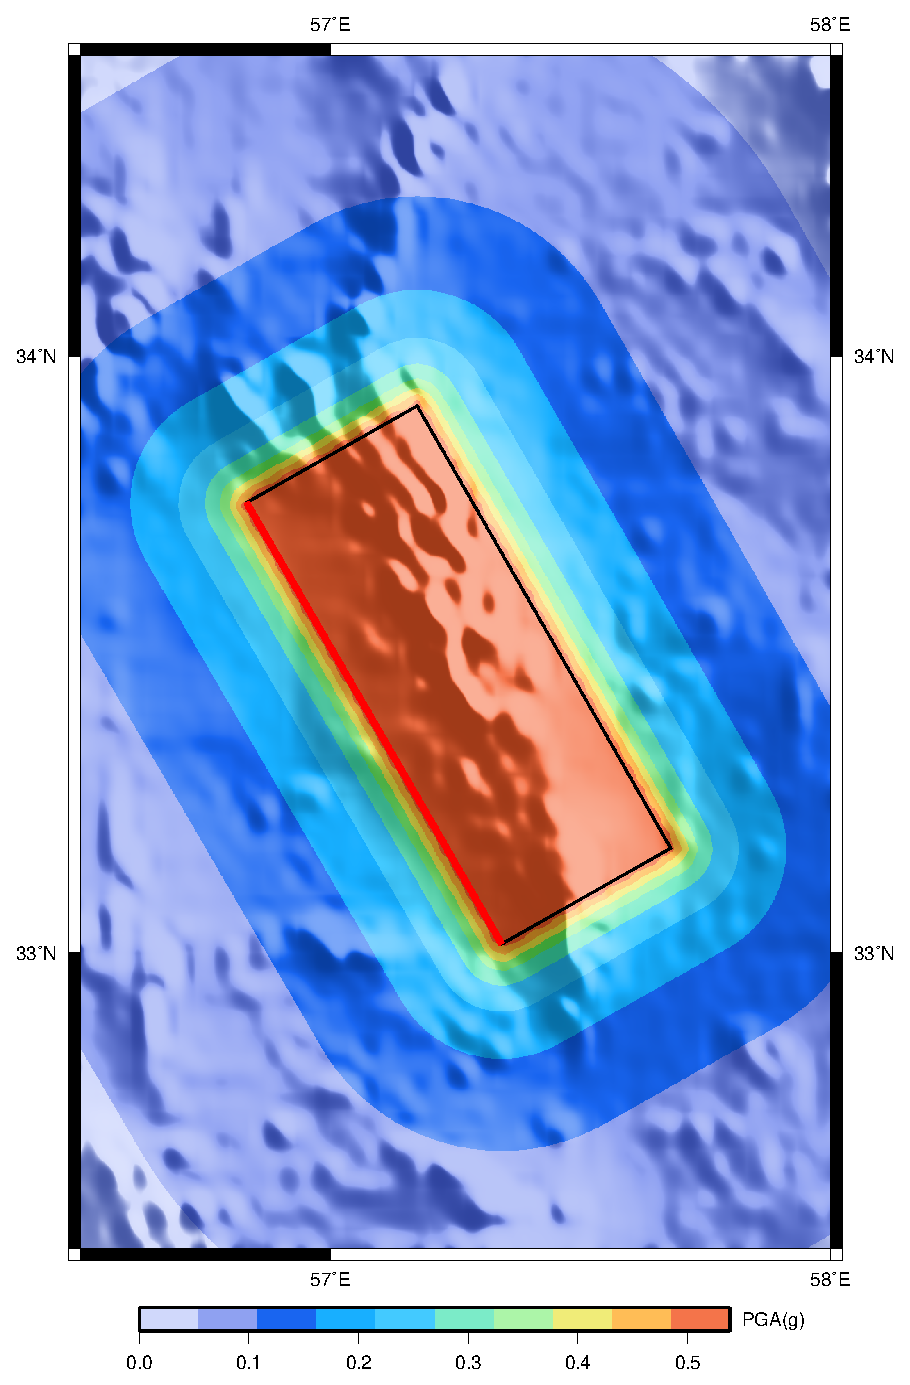
\includegraphics[width=5cm]{./Figures/Part_Hazard/medianGmfTabasPGA.eps}}
\subfigure[]{
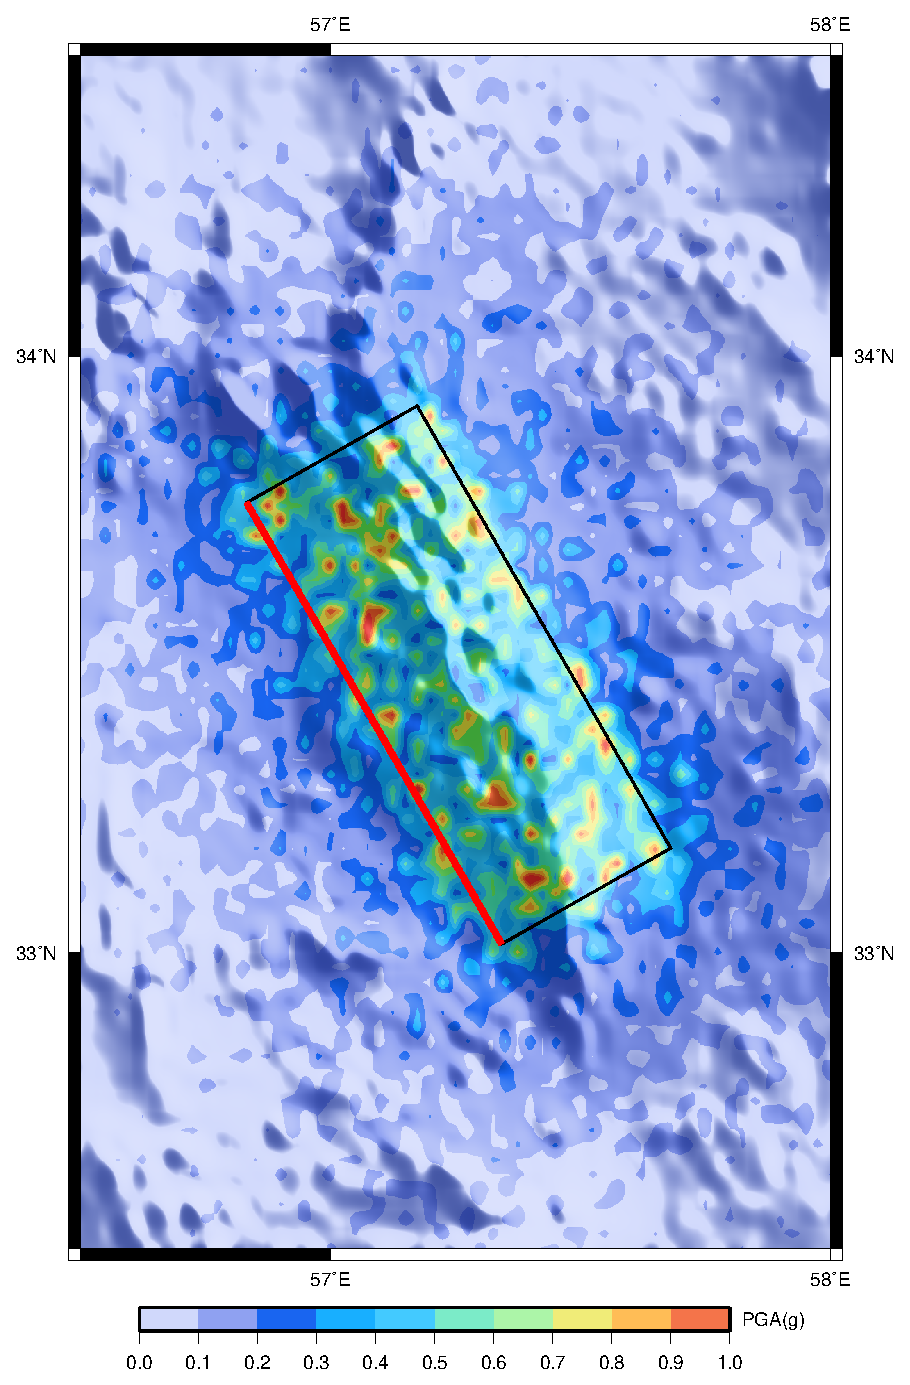
\includegraphics[width=5cm]{./Figures/Part_Hazard/uncorrelatedGmfTabasPGA.eps}}
\subfigure[]{
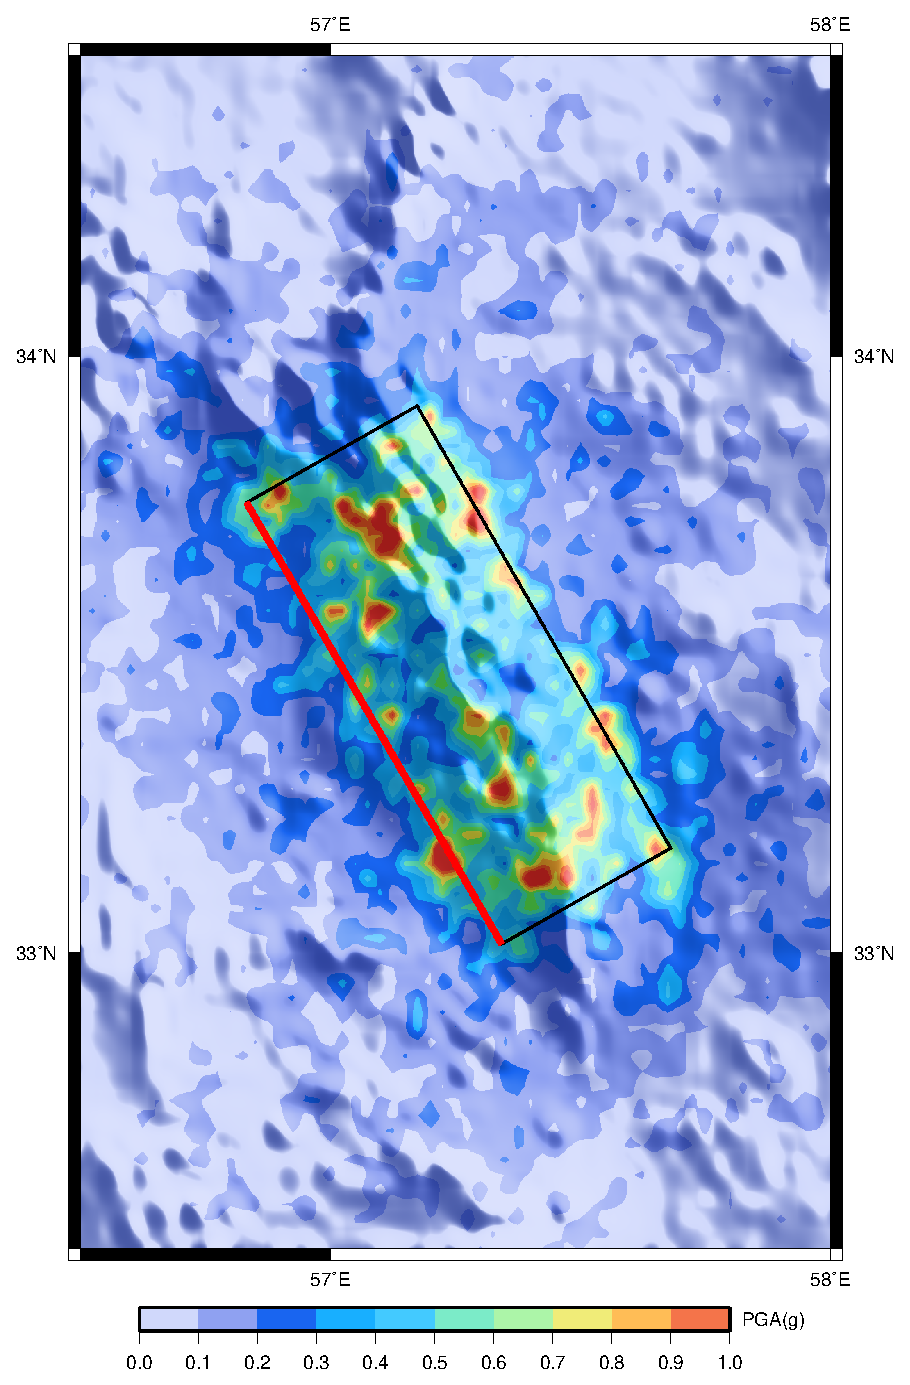
\includegraphics[width=5cm]{./Figures/Part_Hazard/correlatedGmfTabasPGA.eps}}
\subfigure[]{
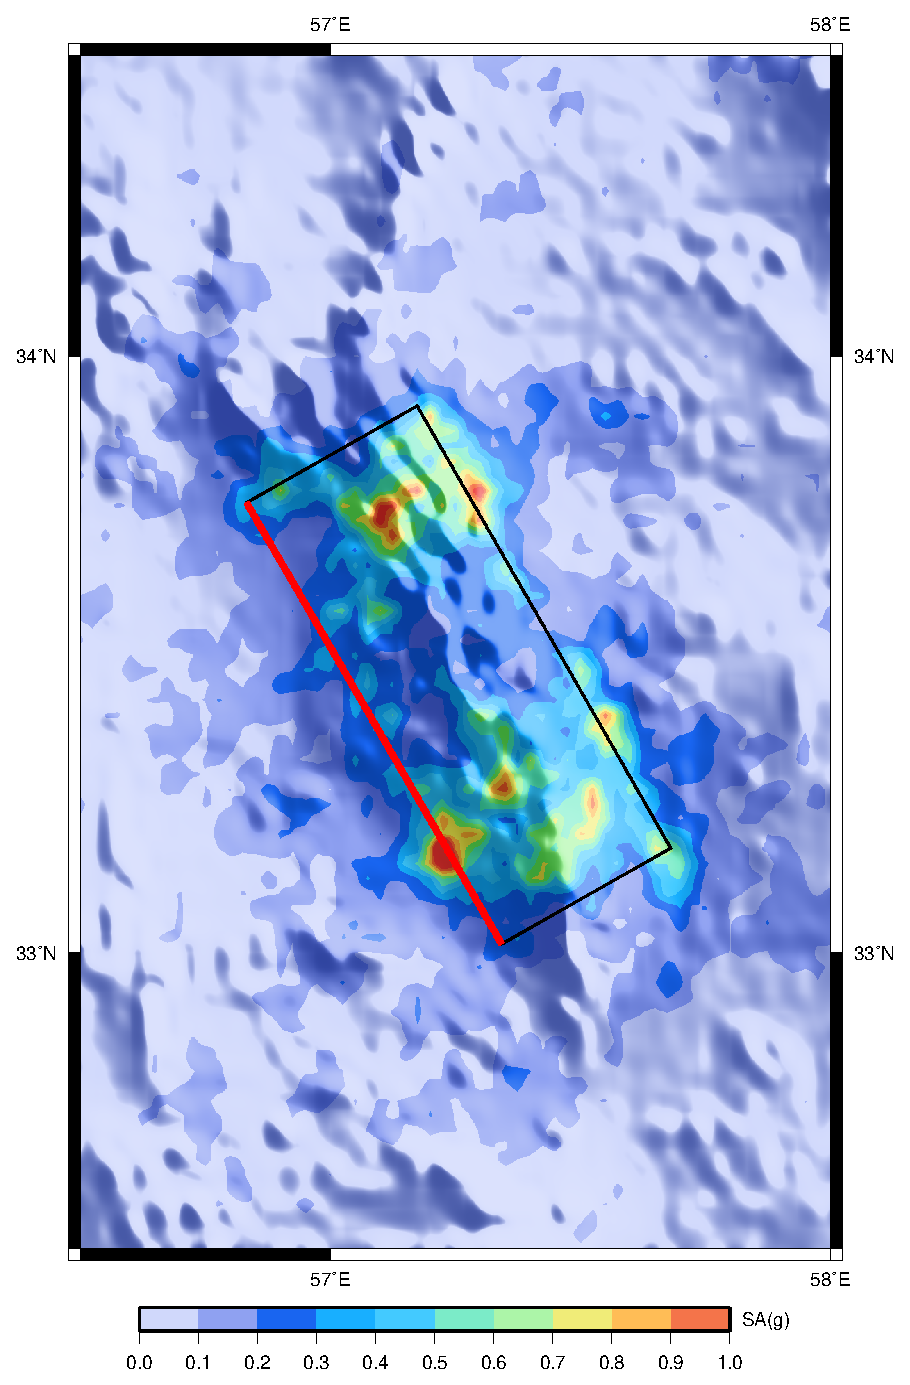
\includegraphics[width=5cm]{./Figures/Part_Hazard/correlatedGmfTabasSA.eps}}
\caption{Examples of median (a), intra-event uncorrelated (b), intra-event 
correlated for PGA (c) and for SA at $T=1$s (d). A rectangular planar rupture 
is considered as source of the shaking (the red line depicts the rupture trace,
and the black line the rupture border). The rupture is associated to a 
magnitude 7 earthquake. The ground motion is estimated using the 
\citet{boore2008} ground motion prediction equation.}
\label{fig:gmfs}
\end{figure}
%
%-------------------------------------------------------------------------------
\clearpage\newpage
\section{PSHA disaggregation}
\label{chap:disaggregation}
%
Seismic hazard disaggregation - or deaggregation - 
\citep{mcguire1995,bazzurro1999} is a procedure aimed at identifying the 
contributions to a specified level of hazard coming from different combinations
of basic variables - such as magnitude and rupture-site distance - 
characterizing the ruptures included in the ERF.
%
Two are the main typologies of disaggregation currently adopted in PSHA 
studies (see for example \citet{petersen2008}): the M-R-$\epsilon$ 
disaggregation and the geographic disaggregation. Conceptually there 
are no differences between the two; simply we can observe that in the 
geographic disaggregation the source-to-rupture distance is replaced by
the position on the topographic surface of the rupture-point used to 
calculate the distance to the site.
%

\subsection{M-D disaggregation}
We start the description of the disaggregation procedure by considering 
the  simplest disaggregation case. 

As a first step we create a container where to progressively store the 
contributions coming from the different ruptures produced by the seismic 
sources contained in the Seismic Source Model.
%
To this purpose, we use a two-dimensional matrix $Q$ with a number or 
rows equal to the number of discrete distance bins and a number of 
columns equal to the number of discrete magnitude intervals. 

The magnitude and distance ranges used to create the $Q$ matrix cover 
the spectrum of values used in the hazard calculation. In particular, 
the magnitude range can be determined considering the properties of 
the seismicity occurrence model for each of the sources contained in
the Seismic Source Model whilst the distance range is implicitly defined
by a maximum integration distance parameter to be specified in the OQ 
configuration file. 
%

The argument of the summation contained in Equation \ref{eq:PSHA_calculation} 
computes the probability of exceedance in a time $t$ of $gm$ generated by the 
occurrence of the rupture $Rup$. Without loss of generality a rupture can be
associated to a magnitude and a source-to-site distance.
% ------------------------------------------------------------------------------
%\chapter{Stochastic event set and ground motion field calculators}
%	The calculation of stochastic event sets and the corresponding ground motion fields is a methodology tightly connected with a specific seismic risk analysis of common use within the insurance and re-insurance industry (CITATION). 
%
OpenQuake given an Earthquake Rupture Forecast can generate a number of seismicity histories, each one representing a possible realisation of the seismicity that the sources included in a Source Model can generate within a given time span (fixed by the user).
% 
The 

Each rupture in a seismicity history is successively associated with a ground motion field, an object describing the spatial distribution of a scalar parameter representative of the intensity of shaking (e.g. PGA or Spectral Acceleration). OpenQuake has the capability to generate 
%
% ------------------------------------------------------------------------------
\section{Stochastic Event Set Calculator}
The Inverse Trasform CITATION is a methodology widely used to randomly sample 
a discrete probabilistic distribution 

%
% ------------------------------------------------------------------------------
\section{Ground Motion Fields calculator} 
We generate ground motion fields using the 
%
%  - - - - - - - - - - - - - - - - - - - - - - - - - - - - - - - - - - - - - - -
\subsection{Spatially correlated ground motion fields}
The genearation of spatially correlated ground motion fields is based on the work of \citet{jayaram2009} where they propose a model - based on a semivarigram - for describing 
\begin{equation}
\gamma(h) = a \left[1-\exp\left(-\frac{3h}{b}\right)\right]
\end{equation}

%
% ------------------------------------------------------------------------------
\section{Stochastic PSHA calculator} 
The OpeQuake stochastic PSHA calculator provides a way to check the consistency between the result provided by a classical PSHA calculator and the results that can be obtained by a number of ground motion fields, representative of the 

% ------------------------------------------------------------------------------
%\chapter{Wesson et al. [2009] risk calculation implementation}
%	%
In the procedure proposed by \cite{wesson2009} the creation of the ERF follows the 
classical approach.

Using an ERF, for each rupture $Rup$ is possible to calculate the 
probability that a given ground motion $U$ is in the interval $u_x\pm \Delta u$ 
given an inter-event variability $\epsilon_{inter}$ (this corresponds to 
equation 3 of \cite{wesson2009}): 
%
\begin{eqnarray}
P(u_x-\Delta u\leq U<u_x+\Delta u|Rup,\epsilon_{inter}) & = &  
	\Phi\bigg(\frac{(\ln (u_x-\Delta u)-\ln(u_0)}{\sigma_{intra}}\bigg) - \nonumber \\
	& - & \Phi\bigg(\frac{(\ln (u_x+\Delta u)-\ln(u_0)}{\sigma_{intra}}\bigg) 
\end{eqnarray}
where $\ln(u_0)$ is the mean of the GMPE computed considering a value 
$\epsilon_{intra}$ and a rupture $Rup$, (generally characterized by a geometry 
and a magnitude) and $\Phi$ is the standard normal CDF. 
  
The next step is to calculate the PMF of losses for a given rupture. Given an asset, 
the probability of suffering a loss value in the interval $[l-\Delta l, l+\Delta[$ 
given a ground motion value in the interval $[u_x-\Delta u,u_x+\Delta u[$ (note that in this 
case the distribution of ground motion $u$ will depend on $\epsilon_{intra}$) 
corresponds to:
%
\begin{equation}
\begin{array}{rl}
P(l-\Delta l\leq L < & l-\Delta l|Rup,\epsilon_{inter}) = \\
 	\sum\limits_{x=0}^{\infty}  
	& P(l-\Delta l\leq L < l-\Delta l|u_x+\Delta u\leq U<u_x+\Delta u) \\
	& P(u_x-\Delta u\leq U<u_x+\Delta u|R,\epsilon_{inter})) \\
\end{array}
\end{equation}
%
If $P^i(L=l|Rup,\epsilon_{inter})$ corresponds to the conditional probability mass
function describing the discrete probability of having a loss in the interval 
$[l-\Delta l, l-\Delta[$ for the asset with index $i$, the probability of cumulated 
losses to a portfolio can be computed as:
\begin{equation}
P_{CL}(CL=cl|M,\epsilon_{inter})=P^1(L=l|Rup,\epsilon_{inter})*\ldots*P^n(L=l|Rup,
	\epsilon_{inter})
\end{equation}
where symbol $*$ stands for convolution. 

Finally, the total probability of exceeding a given level of cumulated losses $cl$ 
computed considering the contributions of all the ruptures occurring on all the 
seismic sources considered is (note that this expression extends equation A10 of
\cite{field2003}):  
%
\begin{equation}
P(CL\geq cl)=1-\prod\limits_{i=1}^{n} 
	\left( 
		1-\sum\limits_{n=1}^{N(i)}
		\sum\limits_{k=-3}^{3}
			P(Rup_{i,n})P(CL\geq cl|Rup_{i,n},\epsilon_k)
	\right)
\end{equation}
where $P(CL\geq cl|Rup_{i,n},\epsilon_k)$ can be simply derived from the PMF 
$P_{CL}(CL=cl|M,\epsilon_{inter})$, $n$ is the number of seismic sources.

% ==============================================================================
% ------------------------------------------------------------------------- Part
\part{Risk}
% ------------------------------------------------------------------------------
\chapter{Introduction}
	%
% ------------------------------------------------------------------------------
\section{OpenQuake-risk: main concepts}
OpenQuake-risk has been developed by the scientific members of the GEM Model Facility, following an extensive review of existing software to calculate seismic risk (\citeauthor{crowleyetal2010} ). It is coded in the Python programming language and is currently linked to OpenQuake-hazard, but there are plans to allow users to input their own hazard in the future.

%
% ------------------------------------------------------------------------------
\section{Calculation Workflows}
OpenQuake currently comprises three risk calculation workflows: one computing losses due to a single event, and the other two computing seismic risk due to most or all of the possible events that might occur in a given region within a certain time span. The calculation workflows are comprised of a number of separate calculators. In order to run any of the calculation workflows, it is necessary to define the geographic coordinates of the region of interest, the type of calculations, the path to the input files, the type of results that are to be produced and several parameters necessary for the hazard calculations. Currently, a configuration file to be provided to OpenQuake incorporates this information.
The following three calculation workflows are thus supported:
\begin{itemize}
\item \textbf{Deterministic Event-Based Risk}: this calculation sequence is capable of computing losses and loss statistics due to a single,
deterministic earthquake, for a collection of assets (see Figure X). Such analyses are of importance, for example, for emergency management planning and for raising societal awareness of risk. 
\item \textbf{Probabilistic Event-Based Risk}: this calculation workflow computes the probability of losses and loss statistics for a collection of
assets, based on the probabilistic hazard (see Figure Y). The losses are calculated with an event-based approach,
such that the simultaneous losses to a set of assets can be calculated.
\item \textbf{Classical PSHA-Based Risk}: this calculation workflow leads to the computation of the probability of losses and loss statistics for
single assets, based on the probabilistic hazard (see Fgure Z). The output of this calculator is useful for
comparative risk assessment between assets at different locations.
\end{itemize}

%\begin{figure}[ht]
%\centering
%\includegraphics[width=9cm,height=9cm]
%\caption{Workflow of the deterministic event-based risk calculations.}
%\label{fig:Scheme_PSHA_calc}
%\end{figure}

%\begin{figure}[ht]
%\centering
%\includegraphics[width=9cm,height=9cm]
%\caption{Workflow of the probabilistic event-based risk calculations.}
%\label{fig:Scheme_PSHA_calc}
%\end{figure}

%\begin{figure}[ht]
%\centering
%\includegraphics[width=9cm,height=9cm]
%\caption{Workflow of the classical PSHA-based risk calculations.}
%\label{fig:Scheme_PSHA_calc}
%\end{figure}

The hazard calculators in the aforementioned workflows have already been described in the hazard section of this book, and so the following chapters focus on the input, the calculators required for the three distinct workflows (deterministic event-based risk calculator, probabilistic event-based risk calculator and classical PSHA-based risk calculator) and the output.
%
% ------------------------------------------------------------------------------
\chapter{OpenQuake Input Description: Risk}
	The two main sources of input information required for a risk calculation with OpenQuake are an exposure model and a vulnerability model (in addition to the calculation type, such as those described in the subsequent chapters, and the region of interest). An exposure model for a given asset category describes, at each location of interest within a given region, the value of each asset typology. The vulnerability model describes the vulnerability characteristics of each asset typology.
%_________________________________________________________
\section{Exposure}
The OpenQuake engine requires an exposure model that needs to be stored according to the respective NRML schema. This file format can withstand several types of exposure elements such as population count, value of dwellings, building count among others. The following parameters are currently being used to describe each asset of the exposure model: 

\begin{itemize}
\item Asset ID: A unique key used to identify the asset instance;
\item Asset description: Brief description of the asset category;
\item Asset value: Numerical value of the quantity of the asset;
\item Location: Geographic coordinates of the asset expressed in decimal degrees.
\end{itemize}

This list of parameters will be further extended in future releases of OpenQuake once more complex data will need to be stored (e.g. value of contents or number of occupants per building).  

\section{Vulnerability}
Vulnerability is defined as the probability distribution of loss, given an intensity measure level. Vulnerability functions can be derived directly, usually through empirical methods where the losses from past events at given locations are related to the levels of intensity of ground motion at those locations, or they can be derived by combining fragility functions and consequence functions. Fragility functions describe the probability of exceeding a set of limit states, given an intensity measure level; limit states describe the limits to performance levels, such as damage or injury levels. Fragility functions can be derived empirically (using observed data) or analytically, by explicitly modeling the behavior of a given asset typology when subjected to increasing levels of ground motion. Consequence functions describe the probability distribution of loss, given a performance level and are generally derived empirically. 
Version 0.2 of OpenQuake only supports vulnerability functions. However, the possibility to describe the vulnerability characteristics of the exposure assets with fragility and consequence functions is planned in OpenQuake such that users can view intermediate results of seismic loss calculations, such as the distribution of damage or injury levels. 

\subsection{Vulnerability Function}
\subsubsection{Discrete Vulnerability Functions}
In the current version of OpenQuake (0.2) discrete vulnerability functions are used to directly estimate human and economic losses in OpenQuake. Discrete vulnerability functions are described by a list of intensity measure levels and corresponding mean loss ratios (ratio of loss to exposed value), associated coefficients of variation and probability distribution. The uncertainty on the loss ratio is assumed in OpenQuake v0.2 to follow a lognormal distribution, however different probabilistic distributions for the uncertainty will be developed in future versions such as the normal or beta distribution. Figure \ref{fig:VFDiscrete} illustrates a discrete vulnerability function.

\begin{figure}[ht]
\centering
\includegraphics[width=11cm,height=7cm]{./Figures/Part_Risk/VFDiscrete.eps}
\caption{Discrete vulnerability function.}
\label{fig:VFDiscrete}
\end{figure}

\subsubsection{Continuous Vulnerability Functions}
In version 0.3 of OpenQuake, continuous vulnerability functions will be implemented. Continuous vulnerability functions are described by continuous distributions of mean loss ratio and coefficient of variation with ground motion intensity. The following figure illustrates this type of functions.

\begin{figure}[ht]
\centering
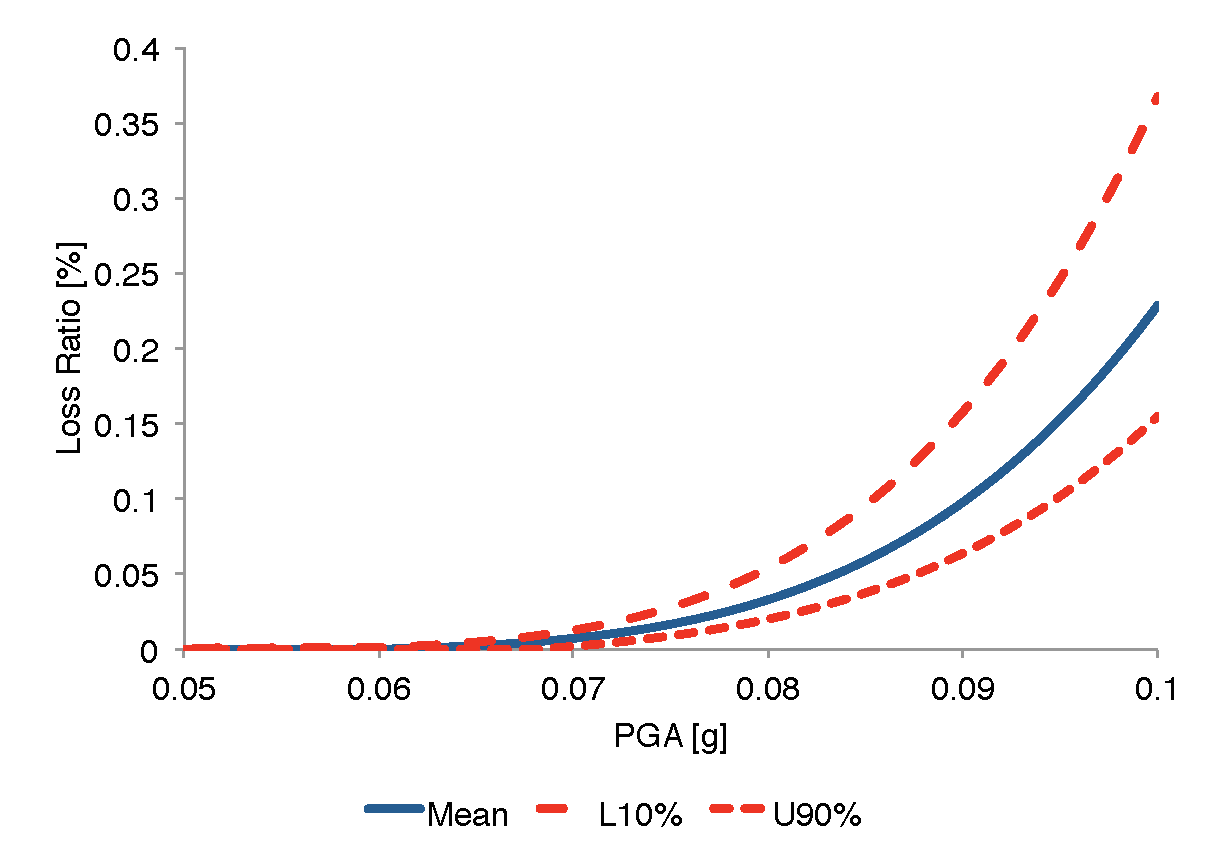
\includegraphics[width=11cm,height=7cm]{./Figures/Part_Risk/VFContinuous}
\caption{Continuous vulnerability function.}
\label{VFContinuous}
\end{figure}

\subsection{Fragility Functions}
Fragility functions describe the probability of exceeding a set of limit states, given an intensity measure level. When the asset category concerns structures (e.g. buildings), the intensity measure can either be structure-independent or structure-dependent. The former can be calculated directly from recorded measurements of ground shaking (e.g. peak ground acceleration, peak ground velocity, spectral acceleration at a given period of vibration, or even macroseismic intensity). The latter requires information on the characteristics of the structures in order to be calculated, for example spectral acceleration at the fundamental period of vibration, or spectral displacement at the limit state period of vibration. The calculation of these characteristics might be through a simple formula (e.g. a yield period-height equation, see e.g. \citet{CrowleyPinho2004} ) or through so-called non-linear static methods, which are needed when the intensity measure is a non-linear response quantity such as spectral displacement at the limit state period of vibration (see e.g. \citet{FEMA440ATC2005}).
Discrete and continuous fragility functions with structure-independent intensity measures aim to be implemented in version 0.3 of OpenQuake. Fragility functions with structure-dependent intensity measures (and the methods necessary to calculate them) will be planned for the version 0.5 release.

\subsubsection{Discrete Fragility Functions}
Fragility functions can be defined in a discrete way by providing for each limit state a list of intensity measure levels and respective probabilities of exceedance. Figure \ref{fig:FFDiscrete} presents a set of discrete fragility functions using a macroseismic intensity.

\begin{figure}[ht]
\centering
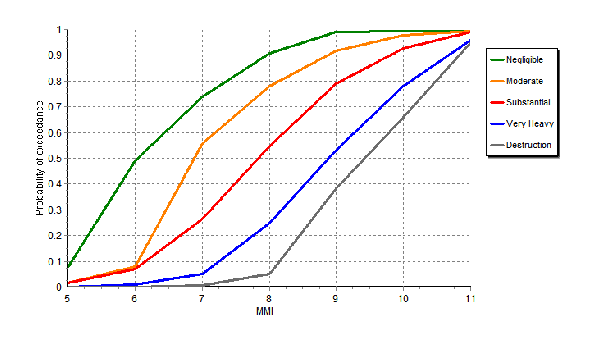
\includegraphics[width=10cm,height=6cm]{./Figures/Part_Risk/FFDiscrete.eps}
\caption{Set of discrete fragility function.}
\label{fig:FFDiscrete}
\end{figure}

\subsubsection{Continuous Fragility Functions}
Continuous fragility functions are defined by the parameters of a cumulative distribution function. The following figure presents an example of a set of continuous fragility functions with a structure-dependent intensity measure.

\begin{figure}[ht]
\centering
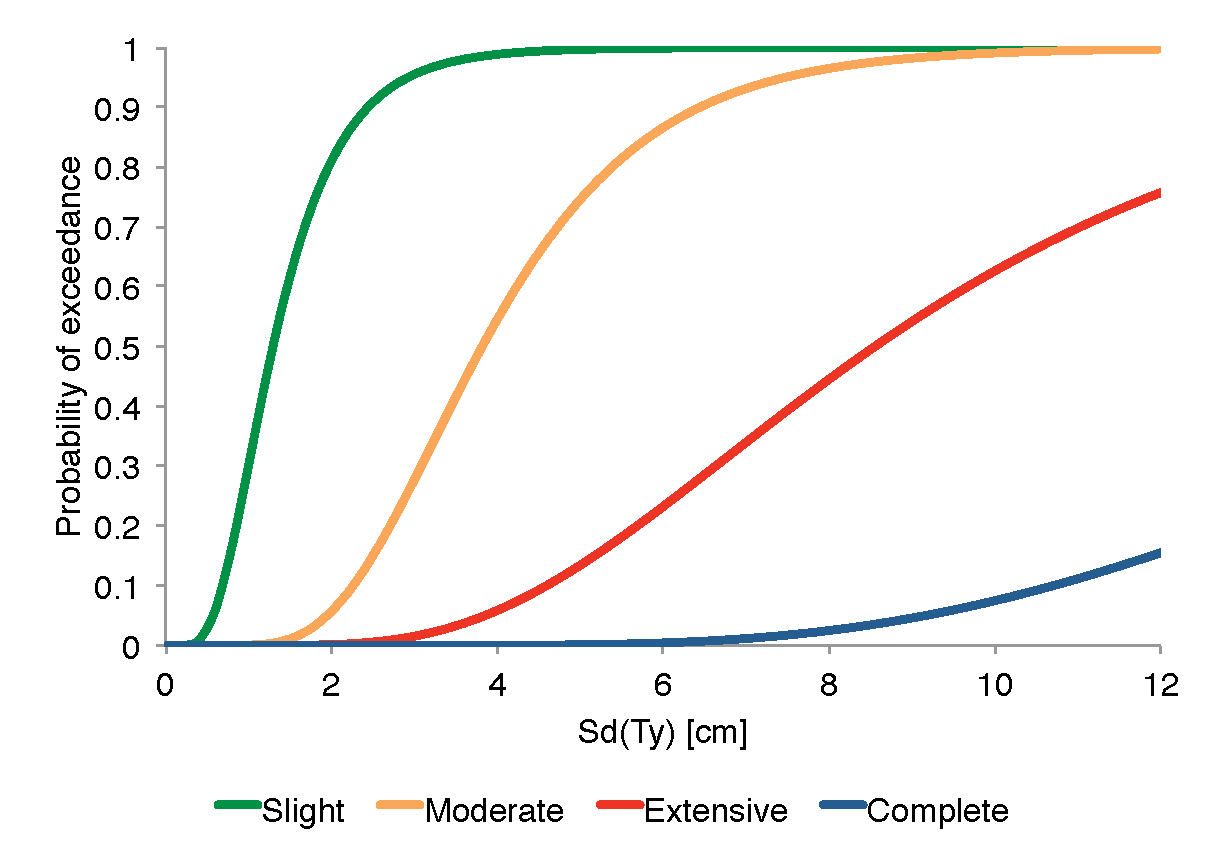
\includegraphics[width=10cm,height=6cm]{./Figures/Part_Risk/FFContinuous.eps}
\caption{Set of continuous fragility function.}
\label{FFcontinuous}
\end{figure}

\subsection{Consequence Functions}
Consequence functions describe the probability distribution of loss, given a performance level. For example, if the asset category is buildings and the performance level is significant damage, the consequence function will describe the mean loss ratio, coefficient of variation and probability distribution. The following figure presents the mean damage ratio for a set of performance levels proposed by two different sources:

\begin{figure}[ht]
\centering
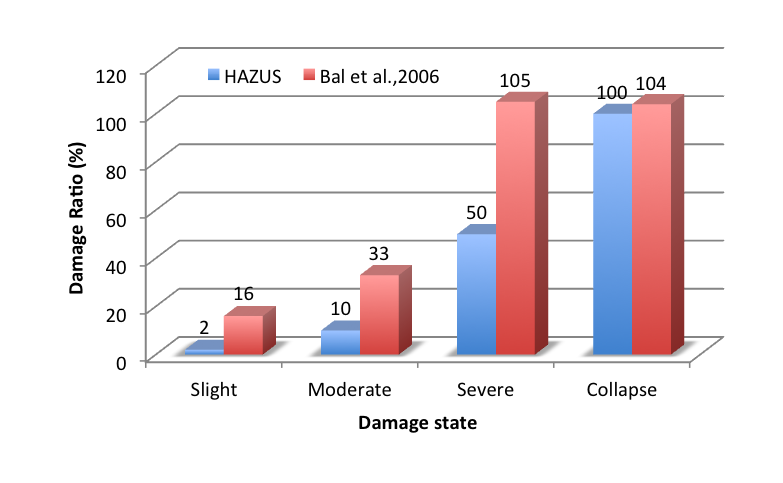
\includegraphics[width=10cm,height=6cm]{./Figures/Part_Risk/ConsequenceFunction.eps}
\caption{Consequence functions adapted from  \citet{Baletal2010}}
\label{ConsequenceFunctions}
\end{figure}


% ------------------------------------------------------------------------------
\chapter{Deterministic Event-Based Risk Calculator}
	

\section{Introduction}
\index{Deterministic Risk}
The deterministic event-based risk calculator is capable of computing losses and loss statistics from a single event for a collection of assets, given a set of ground motion fields. A set of ground motion fields is required to represent the aleatory variability (both inter- and intra-event) in the ground motion prediction equation. The input ground motion fields are currently calculated following the deterministic event-based workflow that has been presented in Figure \ref{fig:Scheme_detrisk_calc}.

For each ground motion field, the intensity measure level at a given site is combined with a vulnerability function, from which a loss ratio is randomly sampled, for each asset contained in the exposure model. The loss ratios that are sampled for assets of a given taxonomy classification at different locations are considered to be either independent or fully correlated, knowing that the reality is likely to lie somewhere in between these two assumptions. Using these results, the mean and standard deviation of the loss ratios across all ground motion fields can be calculated. Loss ratios are converted into losses by multiplying by the value of the asset given in the exposure model. It is furthermore possible to sum the losses throughout the region and to compute the mean and standard deviation of the total loss. 

\section{Calculation Steps}

To compute the mean loss:

\begin{enumerate}
\item For each ground motion field, the intensity measure level at the location of the asset is used to derive the mean loss ratio and associated coefficient of variation from the vulnerability function. Since currently the vulnerability functions are being defined in a discrete manner, it is quite probable that the intensity measure level provided by the ground motion field is not contained in the vulnerability function. In these cases, linear interpolation methods are being employed to derive the mean loss ratio at the intensity measure level of interest. 

\item The engine takes the vulnerability function assigned to each asset and checks if the coefficient of variation is zero. If so, the loss ratios are derived based on the mean loss ratio for each intensity measure level. Otherwise, if the uncertainty is defined, it is randomly sampled following the probabilistic distribution of the respective vulnerability function, as described below:

\begin{equation}
\log{LR_n} = \mu + \epsilon\sigma
\end{equation}

Where $\mu$ and $\sigma$ stand for the mean and standard deviation of the logarithm of the loss ratios respectively and $\epsilon$ is a term that has a standard normal distribution with a zero mean and a standard deviation of one.  

The method used to sample epsilon can follow two approaches depending on whether the correlation between the vulnerability of assets of a given taxonomy is to be considered or not:

\begin{itemize}

\item Perfectly correlated: the term $\epsilon$ is randomly sampled once for the first asset and this result is used to derive the loss ratio for all the assets of the same taxonomy. 

\item Uncorrelated: the term $\epsilon$ is always randomly sampled for each asset and therefore the correlation between the vulnerability of the assets is ignored.

\end{itemize}

It is expected that the true level of correlation lies somewhere between these two assumptions, and thus they provide boundaries to the expected output. 


\item The mean loss ratio for each asset across all possible simulations of the deterministic event can be calculated through the formula:

\begin{equation}
LR=\frac{\sum^m_{n=1}LR_n|IML}{m}
\end{equation}

Where $m$ stands for the number of ground motion fields simulated.

\item The mean loss can then be derived by multiplying the mean loss ratio by the value of the asset contained in the exposure model file.

\end{enumerate}

To compute the standard deviation of the loss:

\begin{enumerate}

\item In order to compute the uncertainty, the engine takes the set of loss ratios for each asset, and computes the associated standard deviation using the classical formula:

\begin{equation}
SD[LR]=\sqrt{  \frac{1}{m}\sum_{n=1}^m{(LR_n-E[LR])^2} }
\end{equation}

Where $E[LR]$ stands for the mean loss ratio computed previously.

\item The standard deviation of the absolute loss can finally be computed by multiplying the standard deviation of the loss ratio by the value of the respective asset.

\end{enumerate}

\section{Calculator Output}
The output of the Deterministic Event-Based Risk Calculator currently comprises loss statistics (mean total loss and standard deviation of total loss) and loss maps. Loss maps are comprised by a set of �loss nodes�, which are associated with a pair of coordinates. For each node, one or more loss values might exist, due to the fact that several different assets can be located at the same location.  Figure \ref{fig:detlosses} presents an example of a loss map containing the expected economic losses for reinforced concrete buildings located in the metropolitan area of Istanbul, considering a rupture of magnitude 7.5Mw under the Sea of Marmara.
\begin{figure}[ht]
\centering
\includegraphics[width=12cm,height=9cm]{./Figures/Part_Risk/LossesDetIstanbul.eps}
\caption{Loss map with the distribution of mean economic losses for reinforced concrete buildings.}
\label{fig:detlosses}
\end{figure} 



% ------------------------------------------------------------------------------
\chapter{Classical PSHA-Based Risk Calculator}
	\section{Introduction}
\index{Probabilistic Risk!PSHA-based}
The Classical PSHA-based risk calculator can be used to calculate loss exceedance curves for single assets, site-by-site, using hazard curves. This calculator thus requires hazard curves as an input, which are currently calculated following the classical PSHA-based workflow that has been presented in Figure \ref{classical_psha_workflow}.

\section{Calculation Steps}

\begin{enumerate}
\item By default, the hazard component of the OpenQuake engine computes the hazard curves for a set of intensity measure levels that are pre-defined in the configuration file. With the integration of the hazard and risk components in the engine, a feature is currently being implemented with the purpose of verifying that this set of values covers the range of intensity measure levels defined in the vulnerability functions. If not, the set of values in which the hazard curves are going to be computed is extended based on the minimum and maximum values of the vulnerability functions.

\item To use this calculator, the hazard curves need first to be converted into probability mass functions (e.g. probability of occurrence of a discrete set of intensity measure levels). To do so, the engine starts by reading the intensity measure levels from the discrete vulnerability functions, and computes the central value between consecutive levels. Two consecutive values define the boundaries of the interval for each intensity measure level and by relating these limits with the hazard curve, the engine computes the corresponding probabilities of exceedance. Figure \ref{fig:ProbOccurrence} contains a discrete vulnerability function (bottom figure) and a hazard curve (top figure) in which the definition of the interval for a given intensity measure level and associated estimation of the probabilities of exceedance of each limit are illustrated. 

\begin{figure}[ht]
\centering
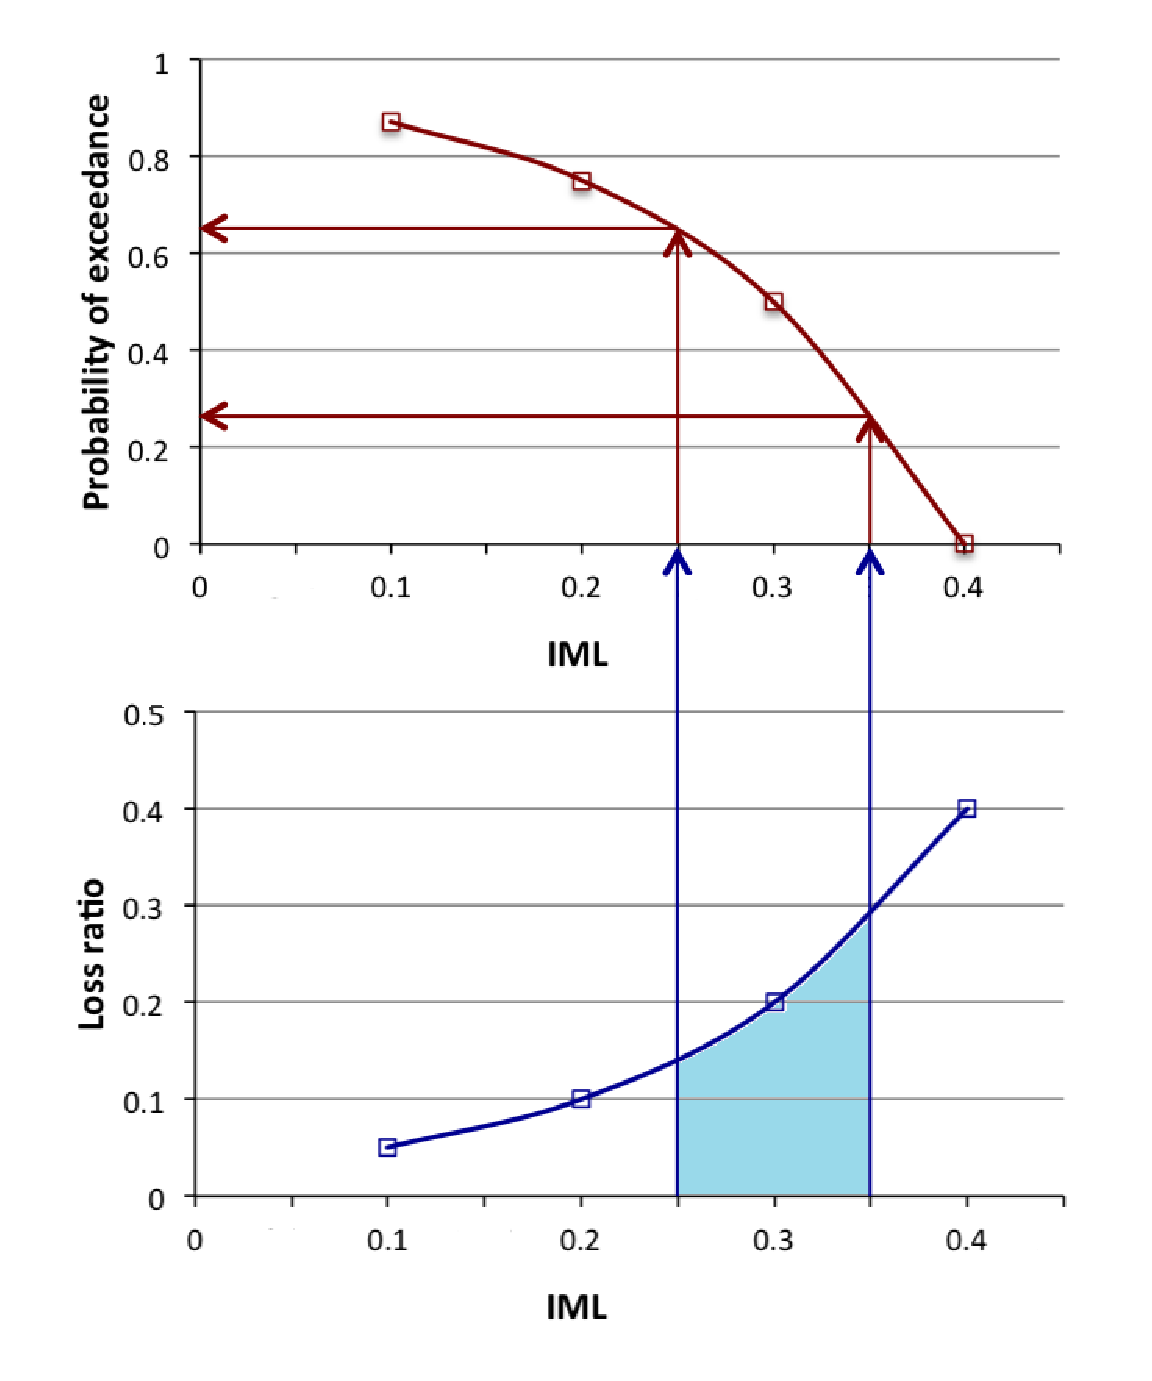
\includegraphics[width=6.5cm,height=7cm]{./Figures/Part_Risk/ProbOccurrence.eps}
\caption{Workflow to estimate the probabilities of exceedance of the boundaries of each intensity measure level.}
\label{fig:ProbOccurrence}
\end{figure}

\item The probability of occurrence of the intensity measure levels that fall within each interval can be derived by subtracting the probabilities of exceedance of the lower and upper limits, as described by the following formula:

\begin{equation}
PO= PE[lower bound]-PE[upper bound]
\end{equation}

\item The discrete vulnerability functions for each asset are converted into loss ratio exceedance matrices (e.g. matrices which describe the probability of exceedance of each loss ratio for a discrete set of intensity measure levels). These matrices have a number of columns equal to the number of intensity measure levels defined on the vulnerability function and a number of rows that can go from the number of loss ratios defined by the discrete function, up to any multiple of this number. In order to properly incorporate the probabilistic distribution of loss ratios per intensity measure level, the probabilities of exceedance should be computed not just for the loss ratios defined on the vulnerability function, but also for many intermediate values between consecutive loss ratios. Currently, following a number of sensitivity analyses, the OpenQuake engine considers 5 intermediate values between consecutive loss ratios, however, this is a parameter that will be adjustable by the user. Figure \ref{fig:LREM} contains an example of a discrete vulnerability function and the respective loss ratio exceedance matrix (in light gray).

\begin{figure}[htb]
\centering
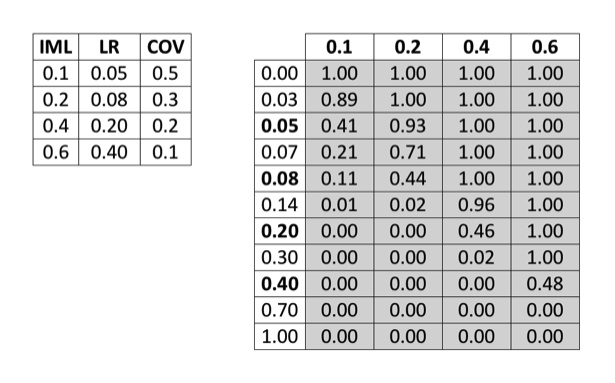
\includegraphics[width=9cm,height=5.5cm]{./Figures/Part_Risk/LREM.eps}
\caption{Example of a discrete vulnerability function and respective loss ratio exceedance matrix.}
\label{fig:LREM}
\end{figure}

Note that for this example only one intermediate value was considered between consecutive loss ratios and in order to consider the whole distribution of the loss ratios, the matrix was computed considering a minimum and maximum loss ratio of 0 and 1 respectively.

\item Finally, each column of the aforementioned matrix is multiplied by the probability of occurrence of the respective intensity measure level (extracted from the hazard curves) to produce a conditional loss ratio exceedance matrix.  Then, for each loss ratio the probabilities of exceedance are summed, leading to a loss ratio exceedance curve, whose set of loss ratios can be multiplied by the value of the asset given by the exposure file to obtain an absolute loss exceedance curve.

\end{enumerate}

\section{Calculator Output}

% ------------------------------------------------------------------------------
\chapter{Probabilistic Event-Based Risk Calculator}
	\section{Introduction}
\index{Probabilistic Risk!Event-Based}
This calculator uses stochastic event sets and associated ground motion fields to compute loss exceedance curves for each asset contained in an exposure model. This calculator thus requires ground motion fields from a number of stochastic events as an input, which are currently calculated following the probabilistic event-based workflow that has been presented in Figure \ref{fig:Scheme_probrisk_calc}.

For each ground motion field, the intensity measure level at a given site is combined with a vulnerability function, from which a loss ratio is randomly sampled, for each asset contained in the exposure model. The loss ratios that are sampled for assets of a given taxonomy classification at different locations are considered to be either independent or fully correlated, knowing that the reality is likely to lie somewhere in between these two assumptions. The occurrence distribution of loss for a given asset is calculated using all of the ground motion fields, leading to a histogram of loss ratios which is then converted into a cumulative histogram, by calculating the number of cumulative occurrences for each interval of loss ratio. The rate of exceedance of each loss ratio is calculated by dividing the number of cumulative occurrences by the number of stochastic event sets multiplied by the length of each event set. By assuming a Poissionian distribution of the occurrence model, the probability of exceedance of each loss ratio is calculated. If a total loss curve for a portfolio of assets is required, a secondary module is used in order to sum the losses from all the assets in the exposure file, per event, before calculating the occurrence distribution of loss. 

\section{Calculation Steps}

\begin{enumerate}
\item The  engine starts by using the set of ground motion fields to extract the intensity measure levels for the location of each asset. 
 
\item Then the engine takes the vulnerability function assigned to each asset and checks if the coefficient of variation is zero. If so, the loss ratios are derived based on the mean loss ratio for each intensity measure level. Otherwise, if the uncertainty is defined, it is randomly sampled following the probabilistic distribution, mean loss ratio and associated coefficient of variation of the respective function, as described below:

\begin{equation}
\log{LR_n} = \mu + \epsilon\sigma
\end{equation}

Where $\mu$ and $\sigma$ stand for the mean and standard deviation of the logarithm of the loss ratios respectively and $\epsilon$ is a term that has a standard normal distribution with a zero mean and a standard deviation of one.  

The method used to sample epsilon can follow two approaches depending on whether the correlation between the vulnerability of assets of a given taxonomy is to be considered or not:

\begin{itemize}

\item Perfectly correlated: the term $\epsilon$ is randomly sampled once for the first asset and this result is used to derive the loss ratio for all the assets of the same taxonomy. 

\item Uncorrelated: the term $\epsilon$ is always randomly sampled for each asset and therefore the correlation between the vulnerability of the assets is ignored.

\end{itemize}

It is expected that the true level of correlation lies somewhere between these two assumptions, and thus they provide boundaries to the expected output. 

\item In this method a histogram of the loss ratios per asset is required. Before the histogram can be built, it is necessary to define the number and width of the bins. The former might vary significantly since it might depend of several factors (e.g. number of ground motion fields, range of ground motion covered by the vulnerability model) while the latter is related with the minimum and maximum values of loss ratio previously computed and with the number of bins. 

\item The histograms for each asset need to be converted into a cumulative histogram. The number of occurrences for each bin can be derived using the following formula:

\begin{equation}
NCO_m = \sum_{n=m} NO_n
\end{equation}

where $NCO_m$ stands for the number of cumulative occurrences of the $m^{th}$ bin of the cumulative histogram and $NO_n$ stands for the number of occurrences of the $n^{th}$ bin of the histogram of the loss ratios.

\item Thereafter, the rate of exceedance of a set of loss ratios needs to be computed for each asset. This set of loss ratios is comprised of the middle values of each bin of the cumulative histogram. The following formula is employed to compute this rate:

\begin{equation}
\lambda(LR_n) = \frac{NCO_n}{TSES}
\end{equation}

Where $\lambda$ stands for the rate of exceedance of the respective loss ratio and $TSES$ stands for the time representative of all stochastic event sets, i.e. the number of stochastic event sets multiplied by the time span of each.

\item Assuming a Poissonion distribution of the occurrence model, the probability of exceedance of the set of loss ratios in a given time span can be derived using the following formula:

\begin{equation}
PE(LR_n) = 1-\exp{-\lambda_n\times t}
\end{equation}

Where $t$ stands for the time span used to produce the stochastic event set.

\end{enumerate}

\section{Calculator Output}
The output of this calculator comprises loss exceedance curves and loss maps. Loss exceedance curves are represented by a list of losses and respective probabilities of exceedance. Furthermore, each curve is associated with a pair of coordinates, an end branch label (that allows the curve to be connected to the set of specifications used in the calculations) and an asset ID (that permits tracking of the asset that each loss curve was computed for). Furthermore, for this calculator, total loss exceedance curves can be produced which combine the losses to all assets into a single loss exceedance curve.  It is noted that cumulative loss exceedance curves, which present the probability of exceedance of cumulative losses within a given time span are not yet supported in OpenQuake. Loss maps for a given probability of exceedance in a given time span can be produced, as well as maps of mean loss within a given time span. Figure \ref{fig:LossCurve} and \ref{fig:ProbLosses} present a total loss exceedance curve and a loss map for a probability of exceedance of 10\% in 50 years for reinforced concrete buildings located in the metropolitan area of Istanbul, respectively. 
\begin{figure}[ht]
\centering
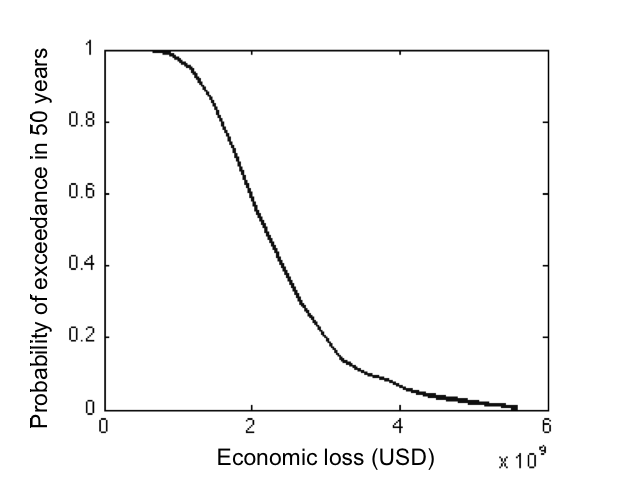
\includegraphics[width=7.5cm,height=6cm]{./Figures/Part_Risk/LossCurveIstanbul.eps} 
\caption{Total loss exceedance curve for RC buildings.}
\label{fig:LossCurve}
\end{figure} 
 \begin{figure}[ht]
\centering
\includegraphics[width=12cm,height=9cm]{./Figures/Part_Risk/LossesProbIstanbul.eps}
\caption{Loss map for a probability of exceedance of 10\% in 50 years.}
\label{fig:ProbLosses}
\end{figure} 

% ==============================================================================
% ------------------------------------------------------------------------- Part
%\part{Socio-Economic Impact Assessment}
%	%
Introduction to the Socio-Economic Impact Assessment

% ==============================================================================
% ------------------------------------------------------------------------- Part
%\part{Modeller's Toolkit}
% ------------------------------------------------------------------------------
%\chapter{Introduction}
%	%
Introduction to the hazard input Modellers' Toolkit

% ------------------------------------------------------------------------------
%\chapter{Input visualization and preparation}
%	%
% ------------------------------------------------------------------------------
\section{Hazard}
%
% ------------------------------------------------------------------------------
\section{Risk}
%
% ------------------------------------------------------------------------------
\section{Socio-Economic Impact}


% ==============================================================================
% ------------------------------------------------------------------------------
% ------------------------------------------------------------------------- Part
%\part{Appendixes}
%\appendix
% ------------------------------------------------------------------------------
%\chapter{nrML}
%	% ------------------------------------------------------------------------------
This is the nrML introduction
%
% . . . . . . . . . . . . . . . . . . . . . . . . . . . . . . . . . . . > Figure
\begin{figure}[!ht]
\small
\begin{Verbatim}[numbers=left,frame=single,fontsize=\small]
<?xml version="1.0" encoding="UTF-8"?>
</ns2:logicTreeSet>
\end{Verbatim}
\normalsize
\caption{nrML example}
\label{fig:nrMl_logic_tree_example}
\vspace*{1em}
\end{figure}
% . . . . . . . . . . . . . . . . . . . . . . . . . . . . . . . . . . . < Figure
%

% ------------------------------------------------------------------------------
%\chapter{Example of OpenQuake risk calculation configuration file}
%	This is a test

% ==============================================================================
% ----------------------------------------------------------------- Bibliography
\bibliographystyle{apalike}
\bibliography{./Bibliography/hazard,./Bibliography/risk,./Bibliography/sei.bib}
% ==============================================================================
% ------------------------------------------------------------------------ Index
\printindex
% ==============================================================================
% ------------------------------------------------------------------- Back Cover
\newgeometry{hmargin={0cm,-0.4cm},height=29.7cm}
\thispagestyle{empty}
\psset{unit=1cm}
\begin{pspicture}(0,0)(21cm,29.7cm)
	\psframe[fillstyle=solid,linecolor=gray02,fillcolor=gray02]
		(0.0cm,0.0cm)(21cm,15.0cm)
	\psframe[fillstyle=solid,linecolor=white,fillcolor=white]
		(0.0cm,15.0cm)(21cm,29.7cm)
	\psframe[fillstyle=solid,linecolor=orange01,fillcolor=orange01]
		(0.0cm,15.0cm)(21cm,15.5cm)
	\psframe[fillstyle=solid,linecolor=orange01,fillcolor=orange01]
		(0.0cm,25.0cm)(21cm,25.1cm)
\end{pspicture}
%
\end{document}
